%%%% APÊNDICE -- DIAGRAMAS DE SEQUÊNCIA E DE FLUXO
%%
%% Reúne os diagramas de sequência e de estado que detalham os protocolos do
%% PRISM, do PRISM Middleware ao streaming Bluetooth do NeuroEstimulator. Os
%% diagramas foram deslocados do Capítulo de Desenvolvimento para preservar a
%% fluidez da leitura textual sem sacrificar o registro detalhado dos
%% protocolos discutidos.

\chapter{Diagramas de sequência e de fluxo dos protocolos do PRISM}\label{cap:apendiceDiagramasSequencia}

Este apêndice reúne, em ordem temática, os diagramas de sequência e de fluxo que detalham os protocolos descritos ao longo do Capítulo~\ref{cap:desenvolvimento}. A reunião dos diagramas em apêndice atende a duas finalidades complementares: preservar, no corpo do texto, uma narrativa contínua sobre cada protocolo, e oferecer ao leitor interessado em uma leitura técnica aprofundada um material consolidado que pode ser consultado de forma autônoma. As referências cruzadas das subseções de origem ao apêndice são feitas individualmente para cada figura, de modo que o leitor possa decidir, a cada ponto da leitura, se prossegue com o texto principal ou se desloca a atenção para o detalhe gráfico.

A organização do apêndice acompanha a estrutura do capítulo. A Seção~\ref{sec:apendiceSeqMiddleware} apresenta os três diagramas que descrevem o \textit{handshake} de quatro fases do PRISM \textit{Middleware}, conforme discutidos na Subseção~\ref{subsec:NPIMiddleware}. A Seção~\ref{sec:apendiceSeqSync} reúne os diagramas associados aos protocolos de troca de dados entre nós, abordados na Subseção~\ref{subsec:NPITrocaDados}. A Seção~\ref{sec:apendiceSeqIRIS} traz os diagramas de estado e de fluxo da camada de orquestração do IRIS \emph{web}, vinculados à discussão da Subseção~\ref{subsubsec:IRISFederacao}. A Seção~\ref{sec:apendiceSeqMobile} apresenta os diagramas que descrevem os fluxos de pareamento, sincronização e etiquetagem do IRIS \textit{Mobile} (Seção~\ref{sec:desenvolvimentoIRISMobile}). Por fim, a Seção~\ref{sec:apendiceSeqStreaming} concentra o diagrama de sequência do protocolo de \textit{streaming} binário do NeuroEstimulator adaptado, complementando a discussão da Subseção~\ref{subsubsec:NEProtocolo}.

% ----------------------------------------------------------------------
\section{Handshake de quatro fases do PRISM Middleware}\label{sec:apendiceSeqMiddleware}
% ----------------------------------------------------------------------

Os cinco diagramas desta seção materializam, em sequência, as três primeiras fases do protocolo de \textit{handshake} entre nós descrito na Subseção~\ref{subsec:NPIMiddleware}. A Fase~1 ocupa um único diagrama, dedicado à abertura do canal cifrado por troca \textit{Elliptic-Curve Diffie--Hellman} (ECDH) sobre a curva NIST P-384 (Figura~\ref{fig:auth-fase-1}). As Fases~2 e~3, por reunirem cada uma duas trocas distintas, foram desdobradas em dois diagramas. A Fase~2 separa o registro inicial do nó (Figura~\ref{fig:auth-fase-2a}), no qual um nó até então desconhecido submete seus metadados ao administrador local, e a identificação propriamente dita (Figura~\ref{fig:auth-fase-2b}), que recupera o nó já cadastrado por meio do \textit{fingerprint} SHA-256 do certificado X.509. A Fase~3 separa a solicitação do desafio aleatório (Figura~\ref{fig:auth-fase-3a}) da resposta assinada com a chave privada RSA-2048, que comprova a posse do certificado e libera a emissão da sessão de aplicação (Figura~\ref{fig:auth-fase-3b}). A quarta fase --- emissão e gestão da sessão de aplicação --- não foi diagramada como sequência por reduzir-se a uma operação de leitura contra o \textit{store} de sessões mantido em Redis, e está descrita textualmente na referida subseção.

\begin{figure}[htpb]
\caption{Abertura de canal criptografado entre nós (Fase~1 do \textit{handshake} do PRISM \textit{Middleware}).}
\label{fig:auth-fase-1}
\centering
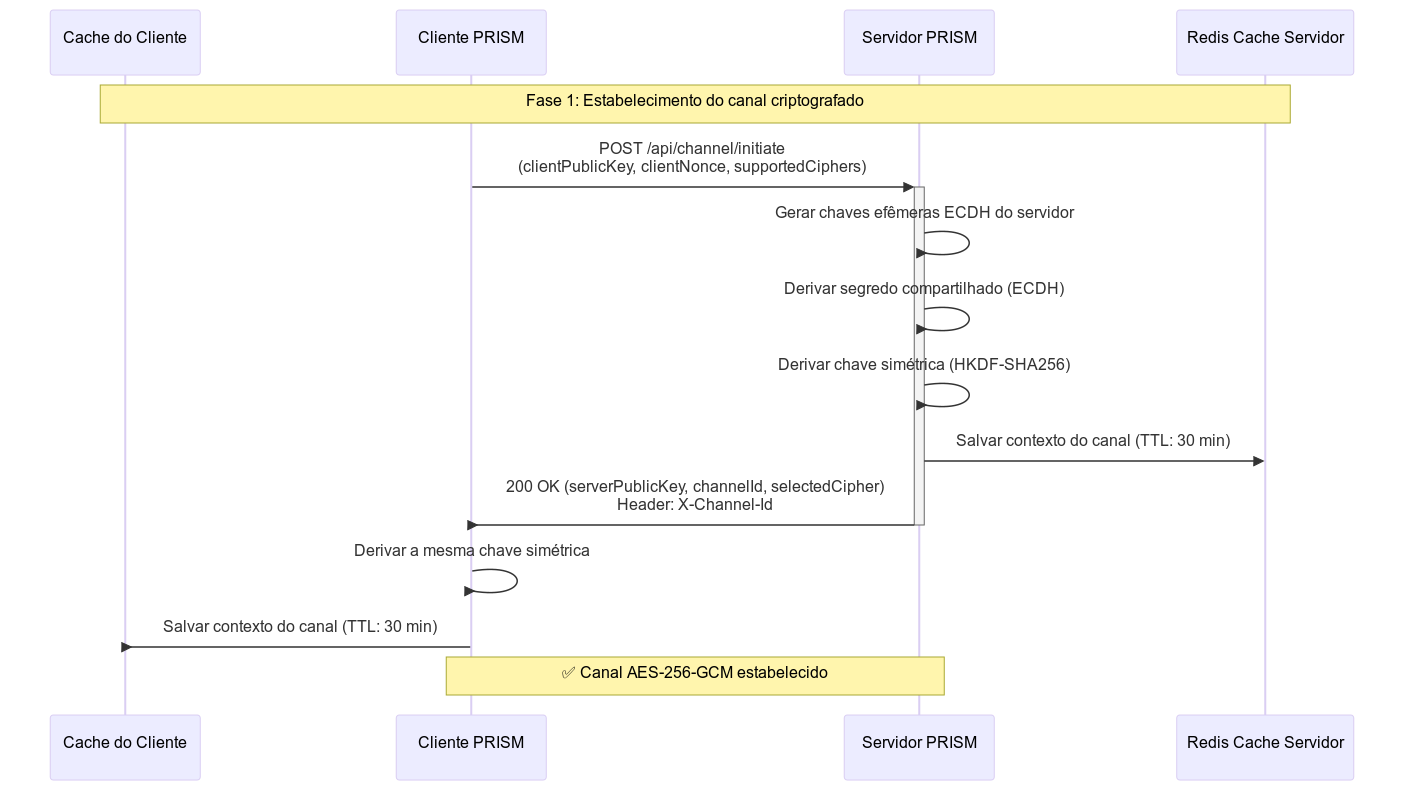
\includegraphics[width=\textwidth]{figuras/Desenvolvimento/auth/fase-1.png}
\fonte{}
\end{figure}

\begin{figure}[htpb]
\caption{Registro do nó (Fase~2A do \textit{handshake} do PRISM \textit{Middleware}).}
\label{fig:auth-fase-2a}
\centering
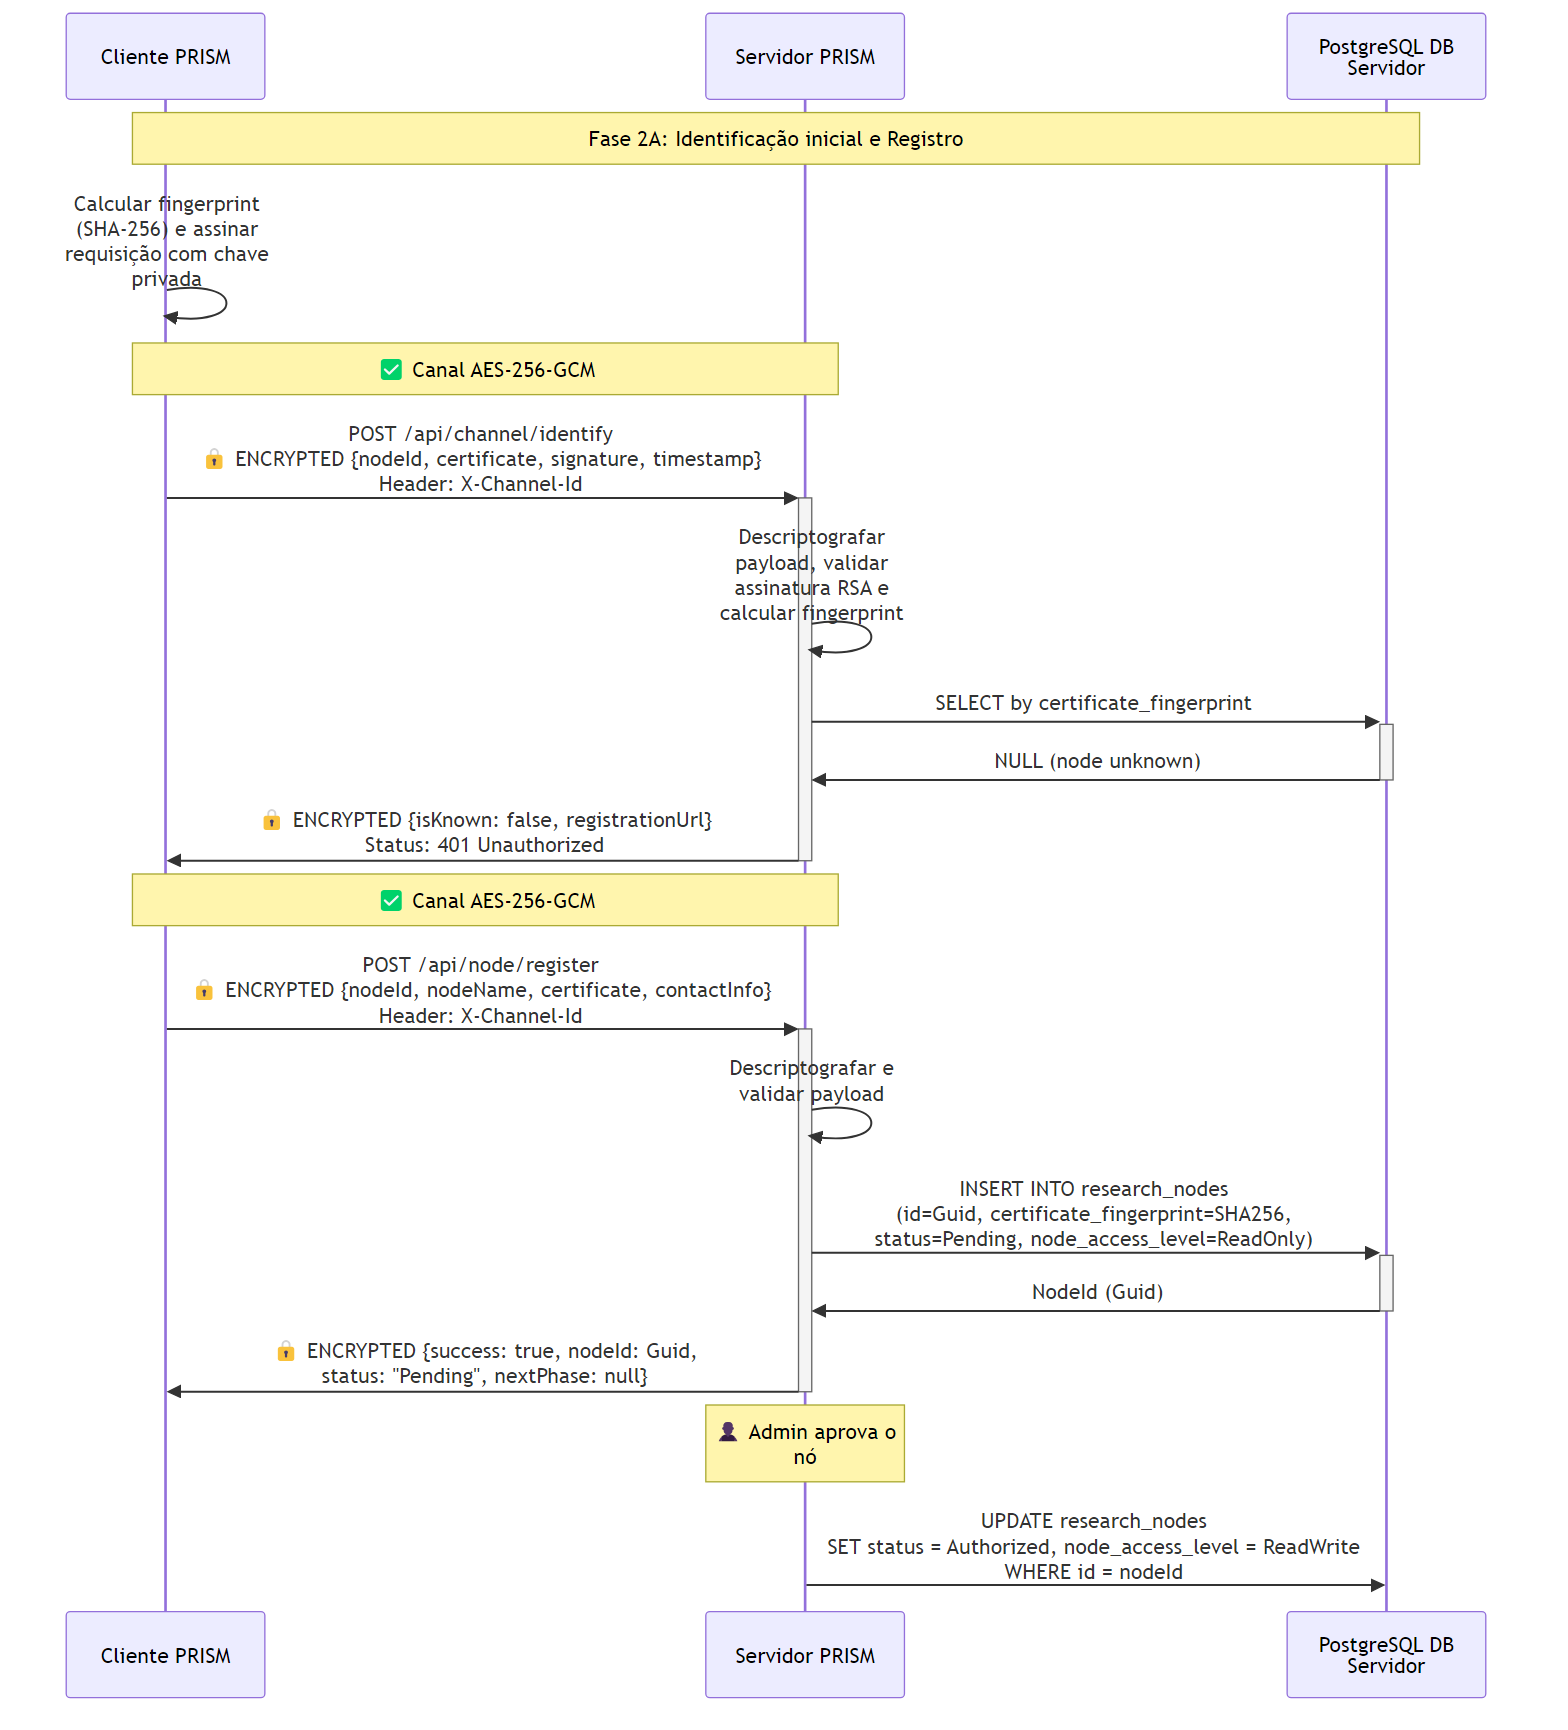
\includegraphics[scale=0.32]{figuras/Desenvolvimento/auth/fase-2a.png}
\fonte{}
\end{figure}

\begin{figure}[htpb]
\caption{Identificação do nó (Fase~2B do \textit{handshake} do PRISM \textit{Middleware}).}
\label{fig:auth-fase-2b}
\centering
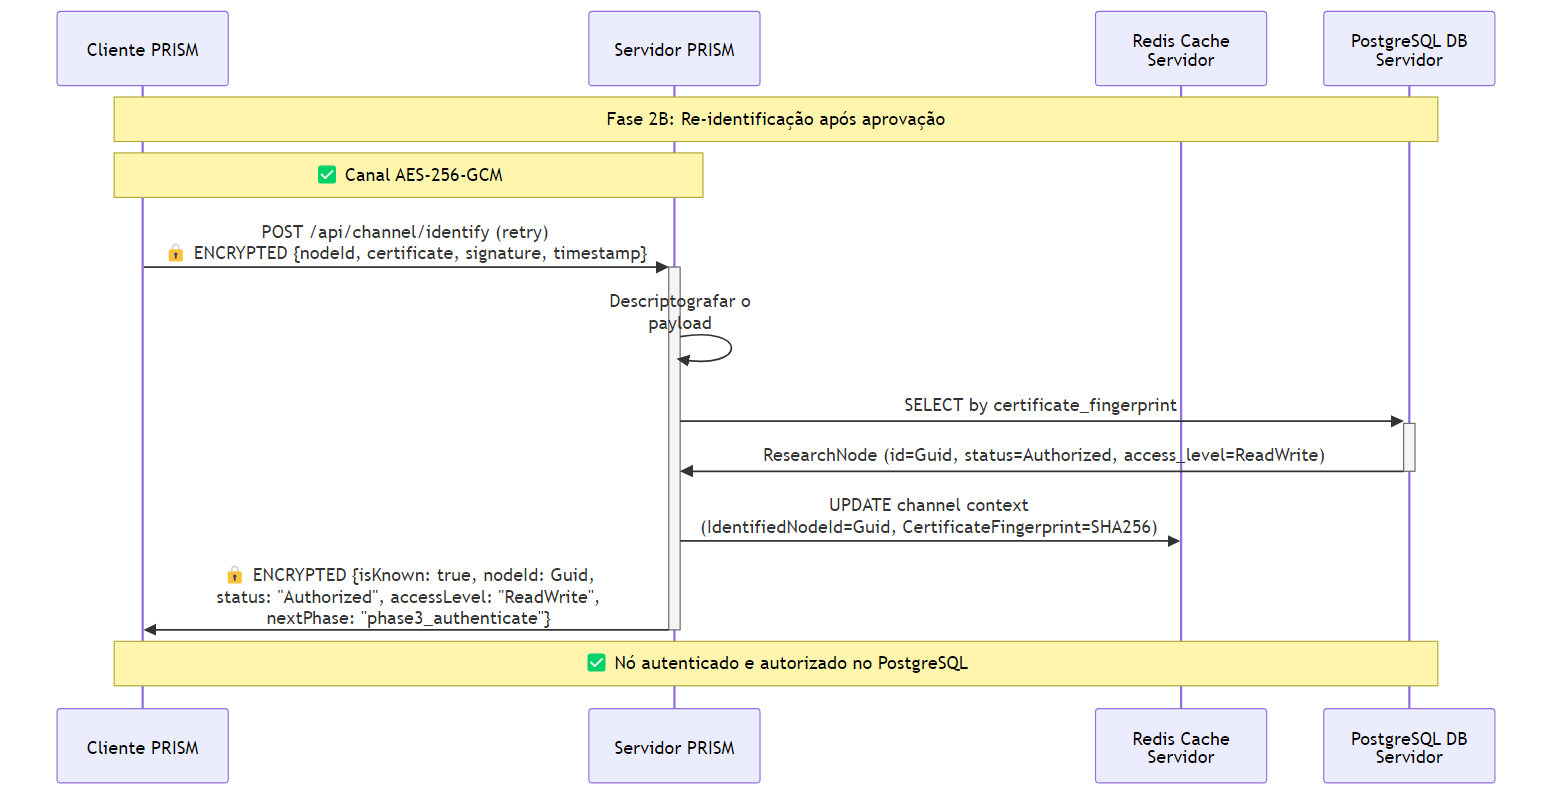
\includegraphics[scale=0.32]{figuras/Desenvolvimento/auth/fase-2b.png}
\fonte{}
\end{figure}

\begin{figure}[htpb]
\caption{Solicitação do desafio (Fase~3A do \textit{handshake} do PRISM \textit{Middleware}).}
\label{fig:auth-fase-3a}
\centering
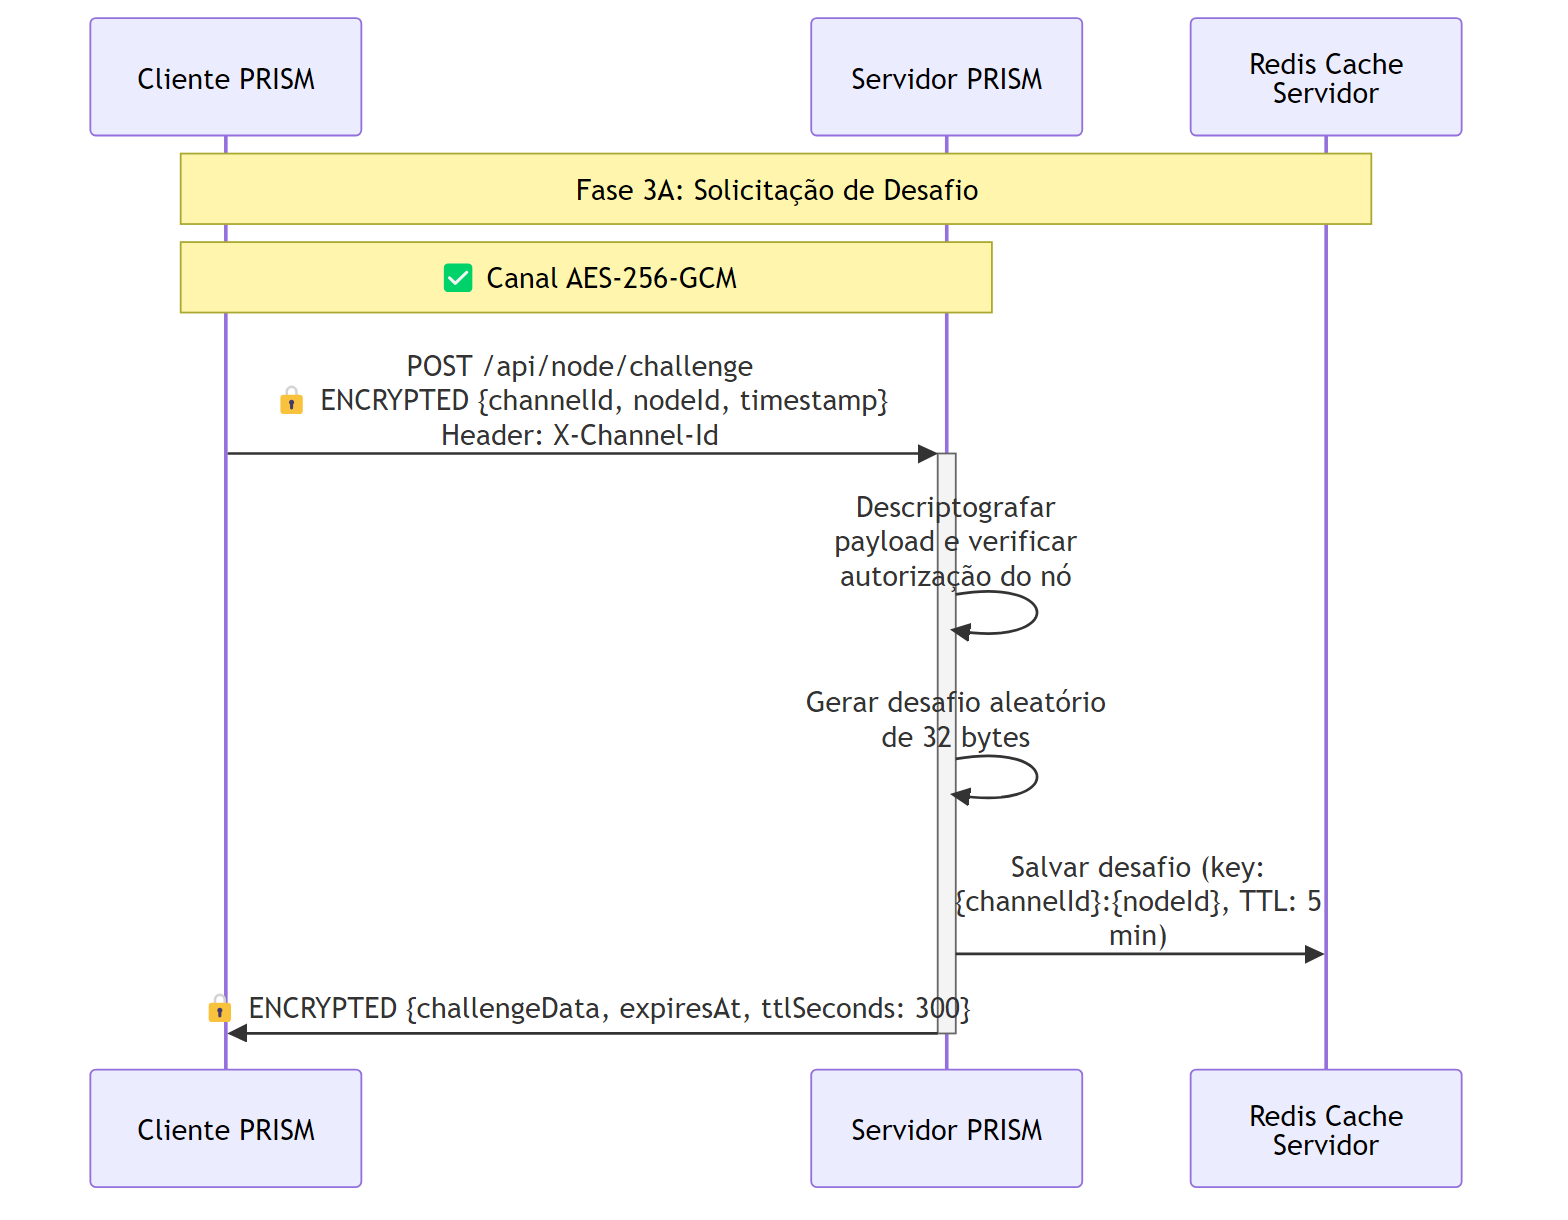
\includegraphics[width=\textwidth]{figuras/Desenvolvimento/auth/fase-3a.png}
\fonte{}
\end{figure}

\begin{figure}[htpb]
\caption{Resposta ao desafio (Fase~3B do \textit{handshake} do PRISM \textit{Middleware}).}
\label{fig:auth-fase-3b}
\centering
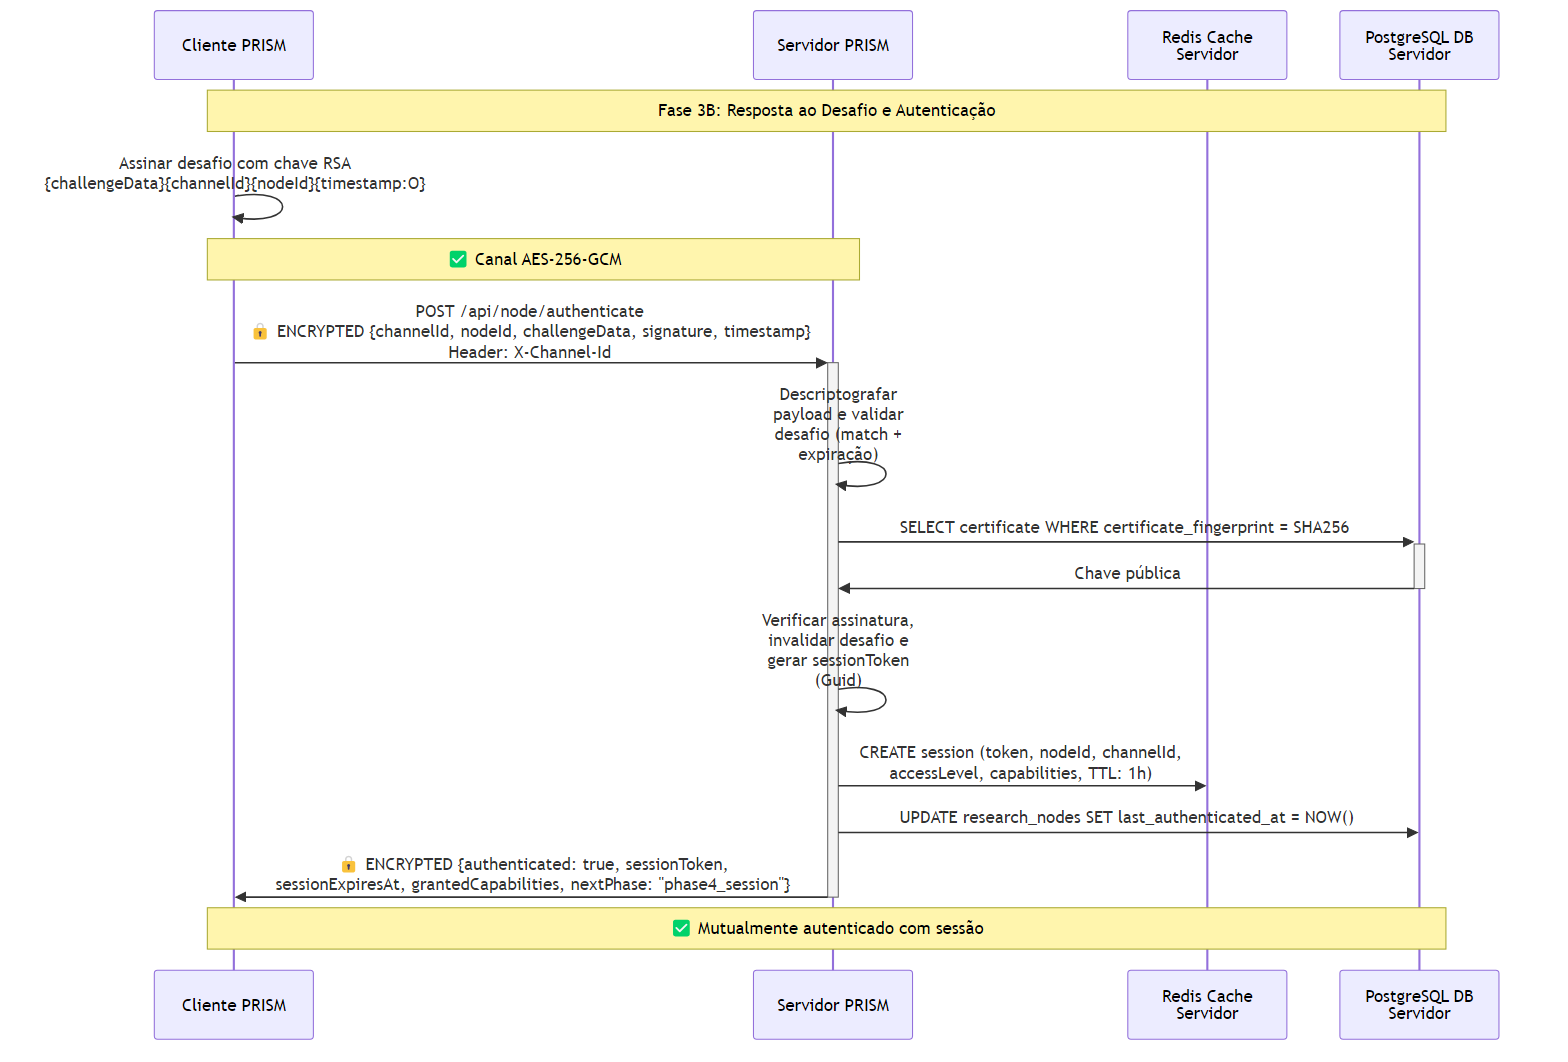
\includegraphics[scale=0.4,angle=90]{figuras/Desenvolvimento/auth/fase-3b.png}
\fonte{}
\end{figure}

\newpage

% ----------------------------------------------------------------------
\section{Sincronização de dados entre nós}\label{sec:apendiceSeqSync}
% ----------------------------------------------------------------------

Esta seção reúne os sete diagramas que detalham os três fluxos centrais discutidos na Subseção~\ref{subsec:NPITrocaDados}: a sincronização incremental do catálogo de rótulos SNOMED CT, decomposta em início, paginação e importação (Figuras~\ref{fig:NPISyncCatalogoInicio}, \ref{fig:NPISyncCatalogoFetch} e~\ref{fig:NPISyncCatalogoImport}); a transferência dos registros de biossinais, decomposta em metadados, conteúdo binário e \textit{commit} transacional (Figuras~\ref{fig:NPISyncBiossinaisMetadados}, \ref{fig:NPISyncBiossinaisBinarios} e~\ref{fig:NPISyncBiossinaisCommit}); e a estratégia de idempotência adotada para que retransmissões não corrompam o estado do nó consumidor (Figura~\ref{fig:NPIIdempotencia}). A decomposição dos dois primeiros fluxos em três diagramas cada deve-se à extensão do diálogo entre os nós envolvidos: ao isolar as etapas de início, transferência e fechamento da transação, busca-se preservar a legibilidade dos diagramas individuais sem sacrificar a representação completa do protocolo.

O fluxo de sincronização do catálogo SNOMED CT é apresentado em três etapas. A Figura~\ref{fig:NPISyncCatalogoInicio} ilustra o início da operação no nó consumidor: a leitura do \textit{watermark} \texttt{LastSyncedAt} no \texttt{SyncLog} local, que delimita o ponto de corte do incremental, e a abertura da transação ACID que envelopa toda a importação subsequente. A Figura~\ref{fig:NPISyncCatalogoFetch} detalha os dois \textit{loops} aninhados percorridos pelo protocolo --- o externo, sobre as quatro famílias de entidades SNOMED, e o interno, sobre as páginas de cada tipo --- responsáveis pela coleta paginada das entidades atualizadas no nó produtor. A Figura~\ref{fig:NPISyncCatalogoImport} fecha o ciclo com o \textit{upsert} idempotente das entidades recebidas e o \textit{commit} da transação local, que materializa a atualização do \textit{watermark}.

O fluxo de transferência dos biossinais segue a mesma estrutura tripartite. A Figura~\ref{fig:NPISyncBiossinaisMetadados} explicita a transferência paginada dos metadados de \texttt{RecordingSession}, incluindo \texttt{Records}, \texttt{RecordChannels} e anotações, com paginação por \textit{cursor} sobre o atributo \texttt{UpdatedAt}. A Figura~\ref{fig:NPISyncBiossinaisBinarios} apresenta a recuperação individualizada dos arquivos binários por canal e o respectivo \textit{upload} ao \textit{blob storage} local, etapa que opera de forma desacoplada da transferência dos metadados. A Figura~\ref{fig:NPISyncBiossinaisCommit} encerra o fluxo com o \textit{commit} transacional bem-sucedido e, no ramo alternativo, a ação compensatória que remove os \textit{blobs} já enviados quando qualquer subetapa do lote falha, garantindo que o nó consumidor jamais persista um estado parcial.

Por fim, a Figura~\ref{fig:NPIIdempotencia} percorre três tentativas consecutivas sobre uma mesma entidade, demonstrando como a combinação entre \textit{Universally Unique Identifier} (UUID) como chave global e \textit{watermark} \texttt{UpdatedAt} torna a retransmissão integral de um lote já aplicado uma operação \textit{no-op} sob a perspectiva de estado.

\begin{figure}[htpb]
\caption{Sincronização incremental do catálogo SNOMED CT --- início: leitura do \textit{watermark} e abertura da transação.}
\label{fig:NPISyncCatalogoInicio}
\centering
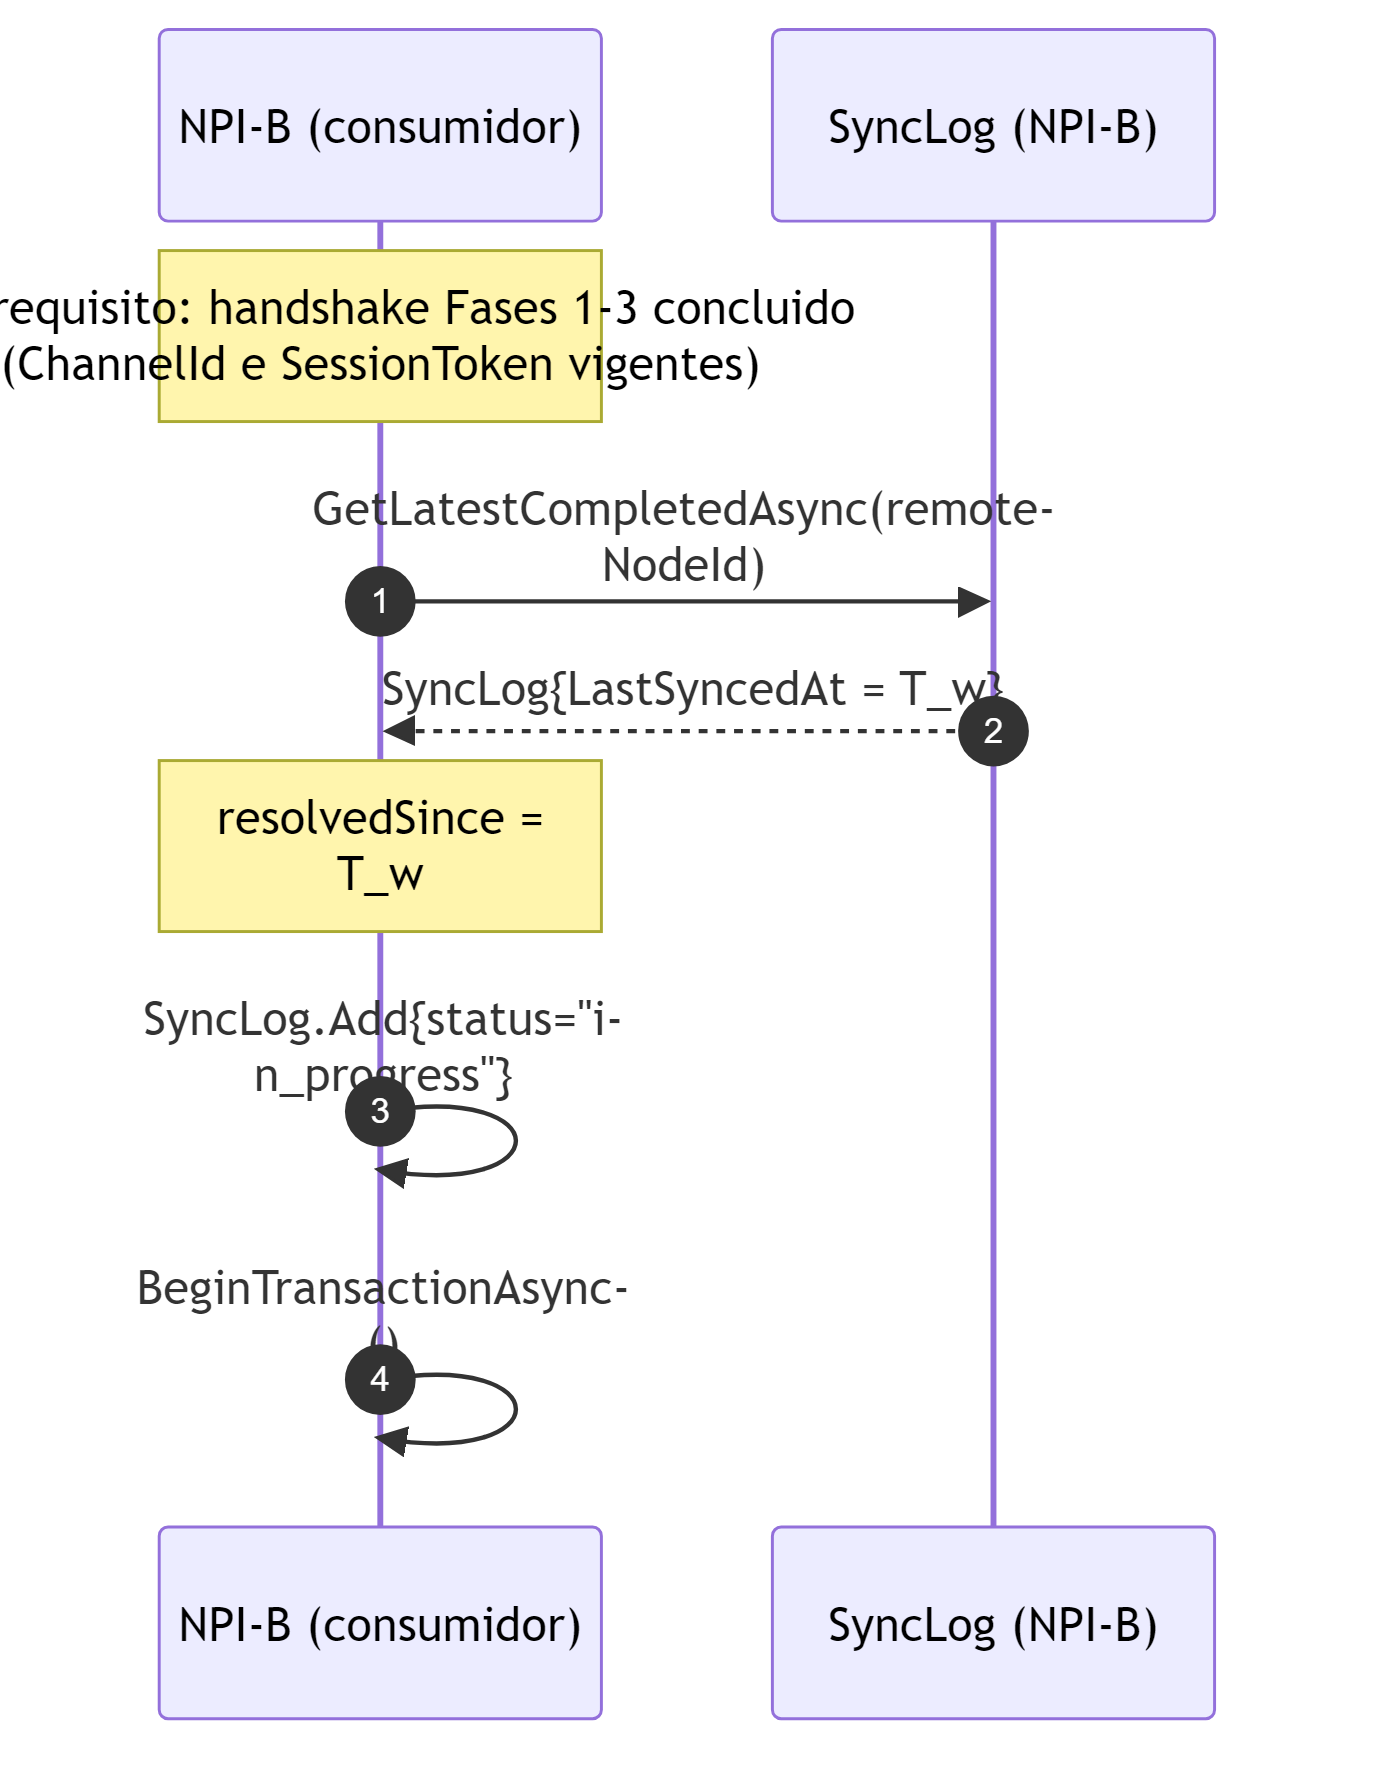
\includegraphics[scale=0.2]{figuras/Desenvolvimento/NPI/sync-catalogo-1-inicio.png}
\fonte{}
\end{figure}

\begin{figure}[htpb]
\caption{Sincronização incremental do catálogo SNOMED CT --- \textit{loops} aninhados de paginação por tipo de entidade.}
\label{fig:NPISyncCatalogoFetch}
\centering
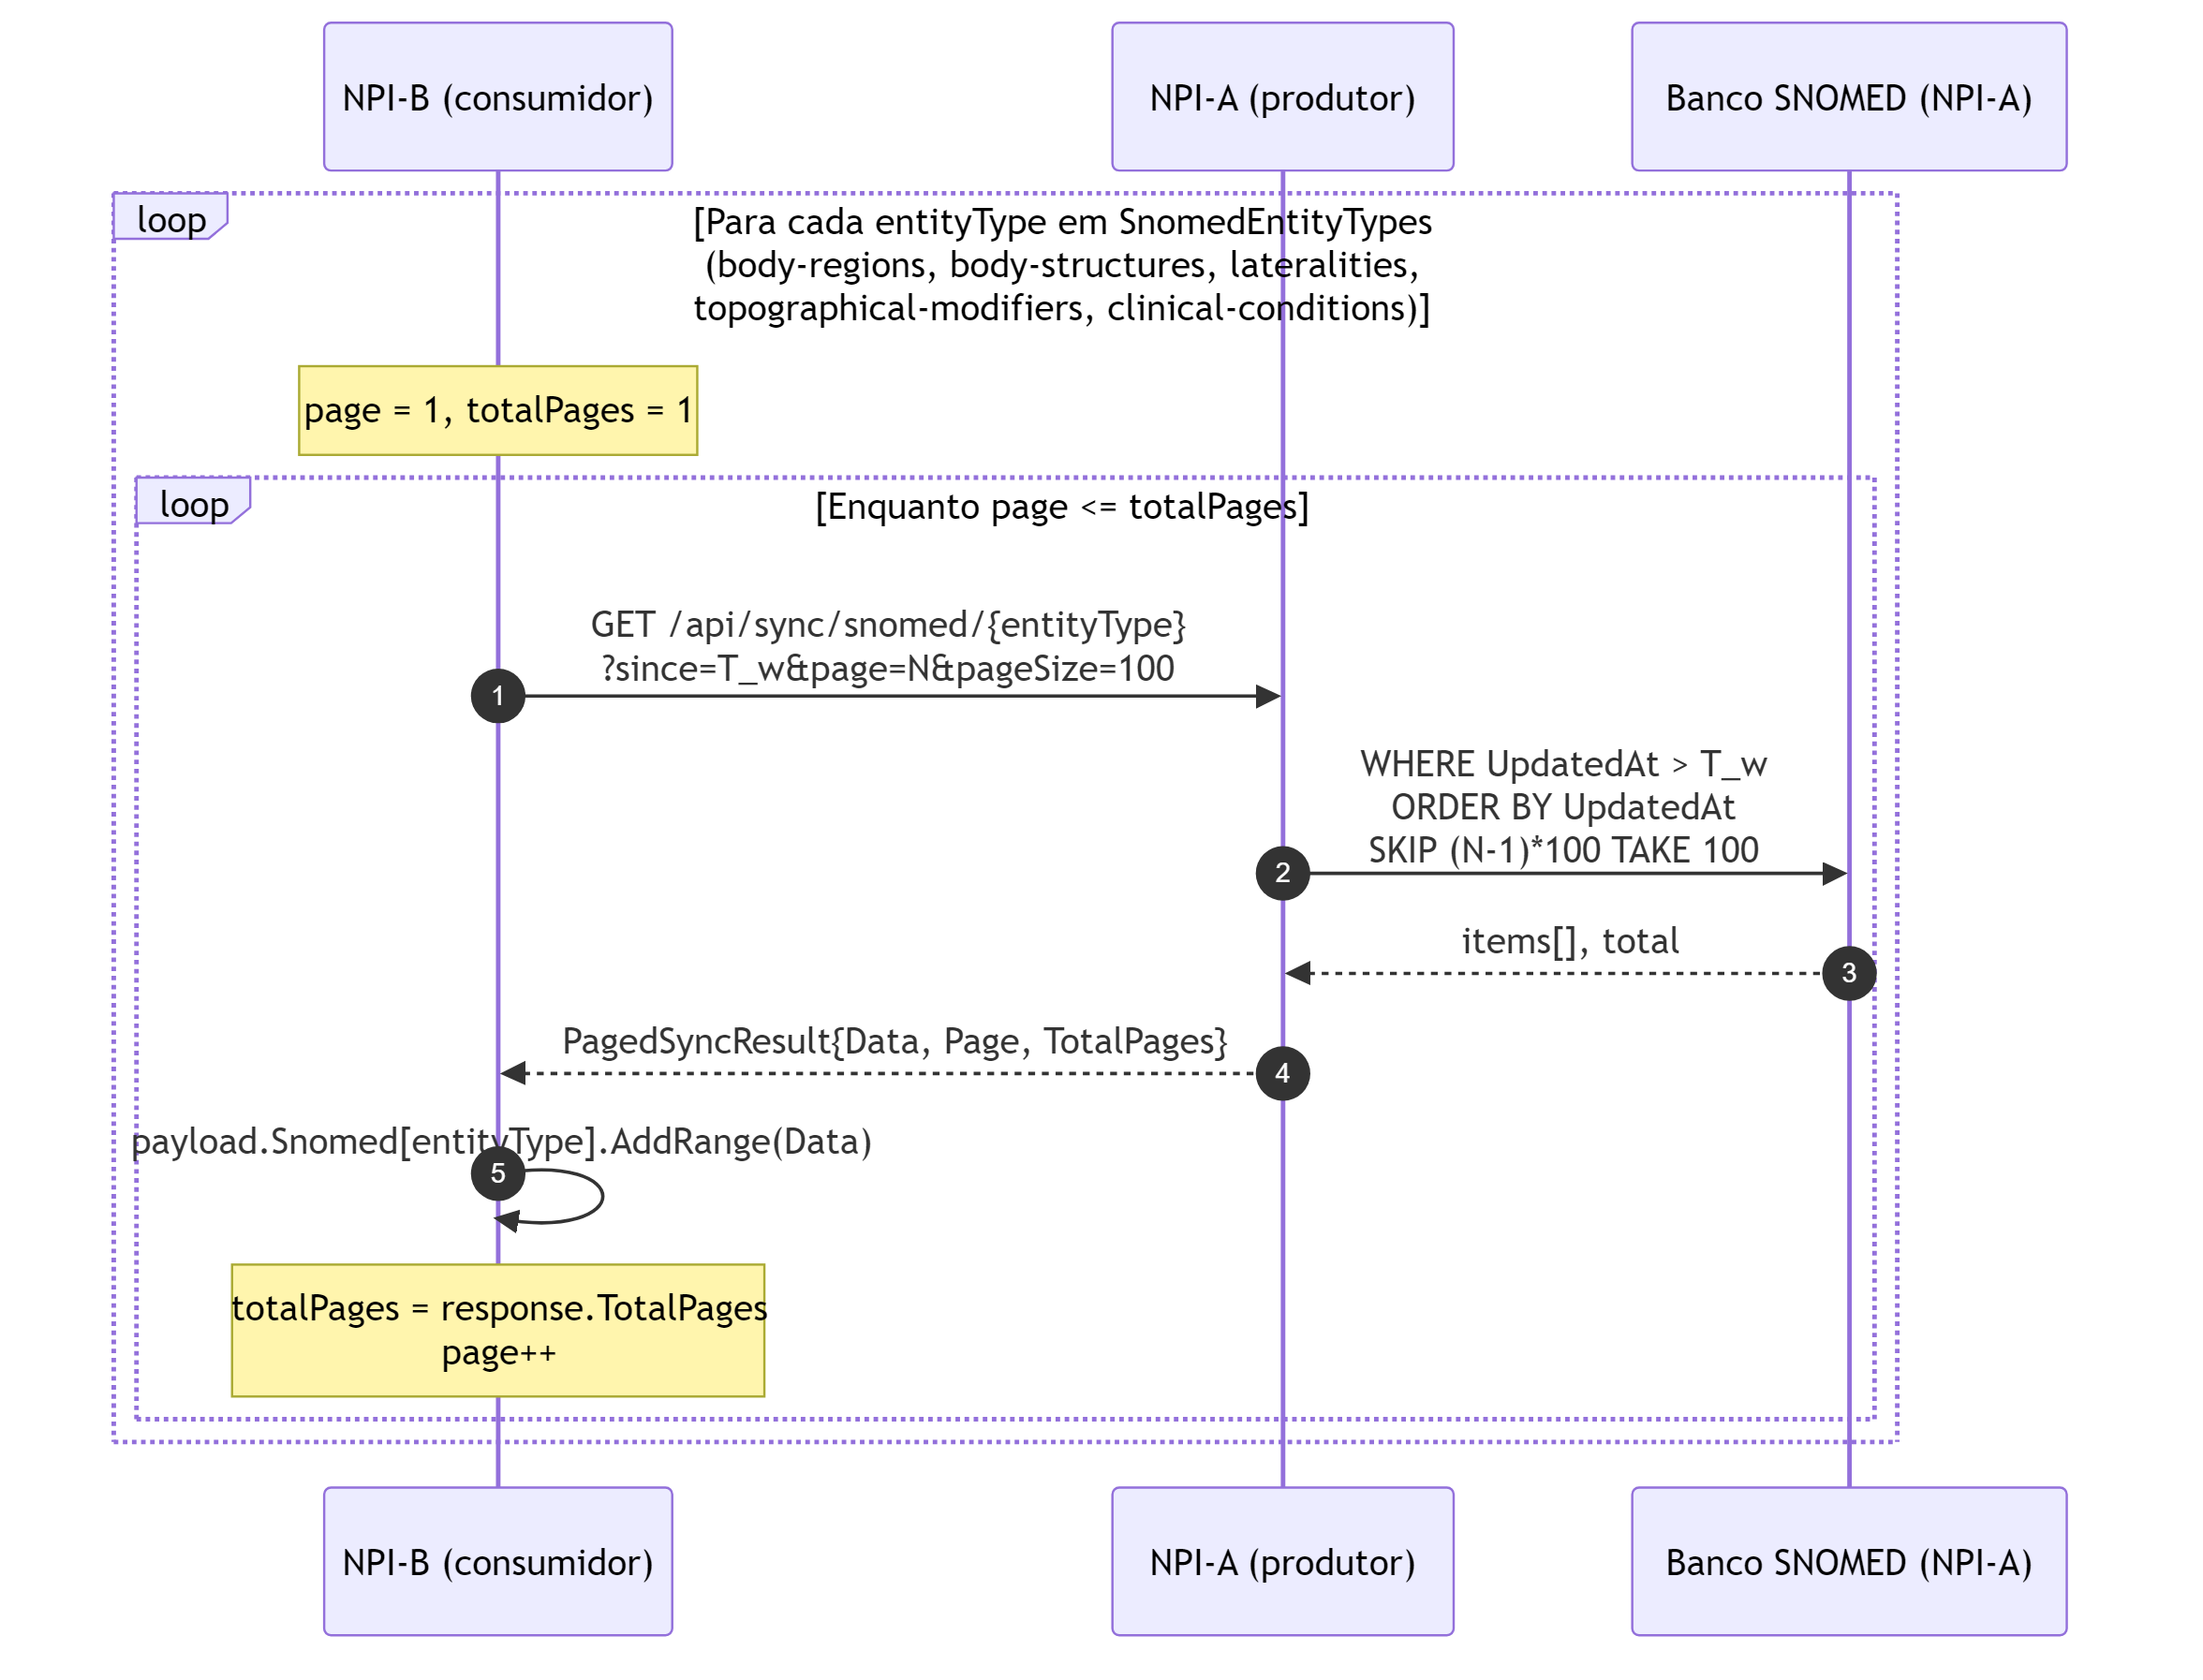
\includegraphics[width=\textwidth]{figuras/Desenvolvimento/NPI/sync-catalogo-2-fetch.png}
\fonte{}
\end{figure}

\begin{figure}[htpb]
\caption{Sincronização incremental do catálogo SNOMED CT --- \textit{upsert} idempotente e \textit{commit} da transação.}
\label{fig:NPISyncCatalogoImport}
\centering
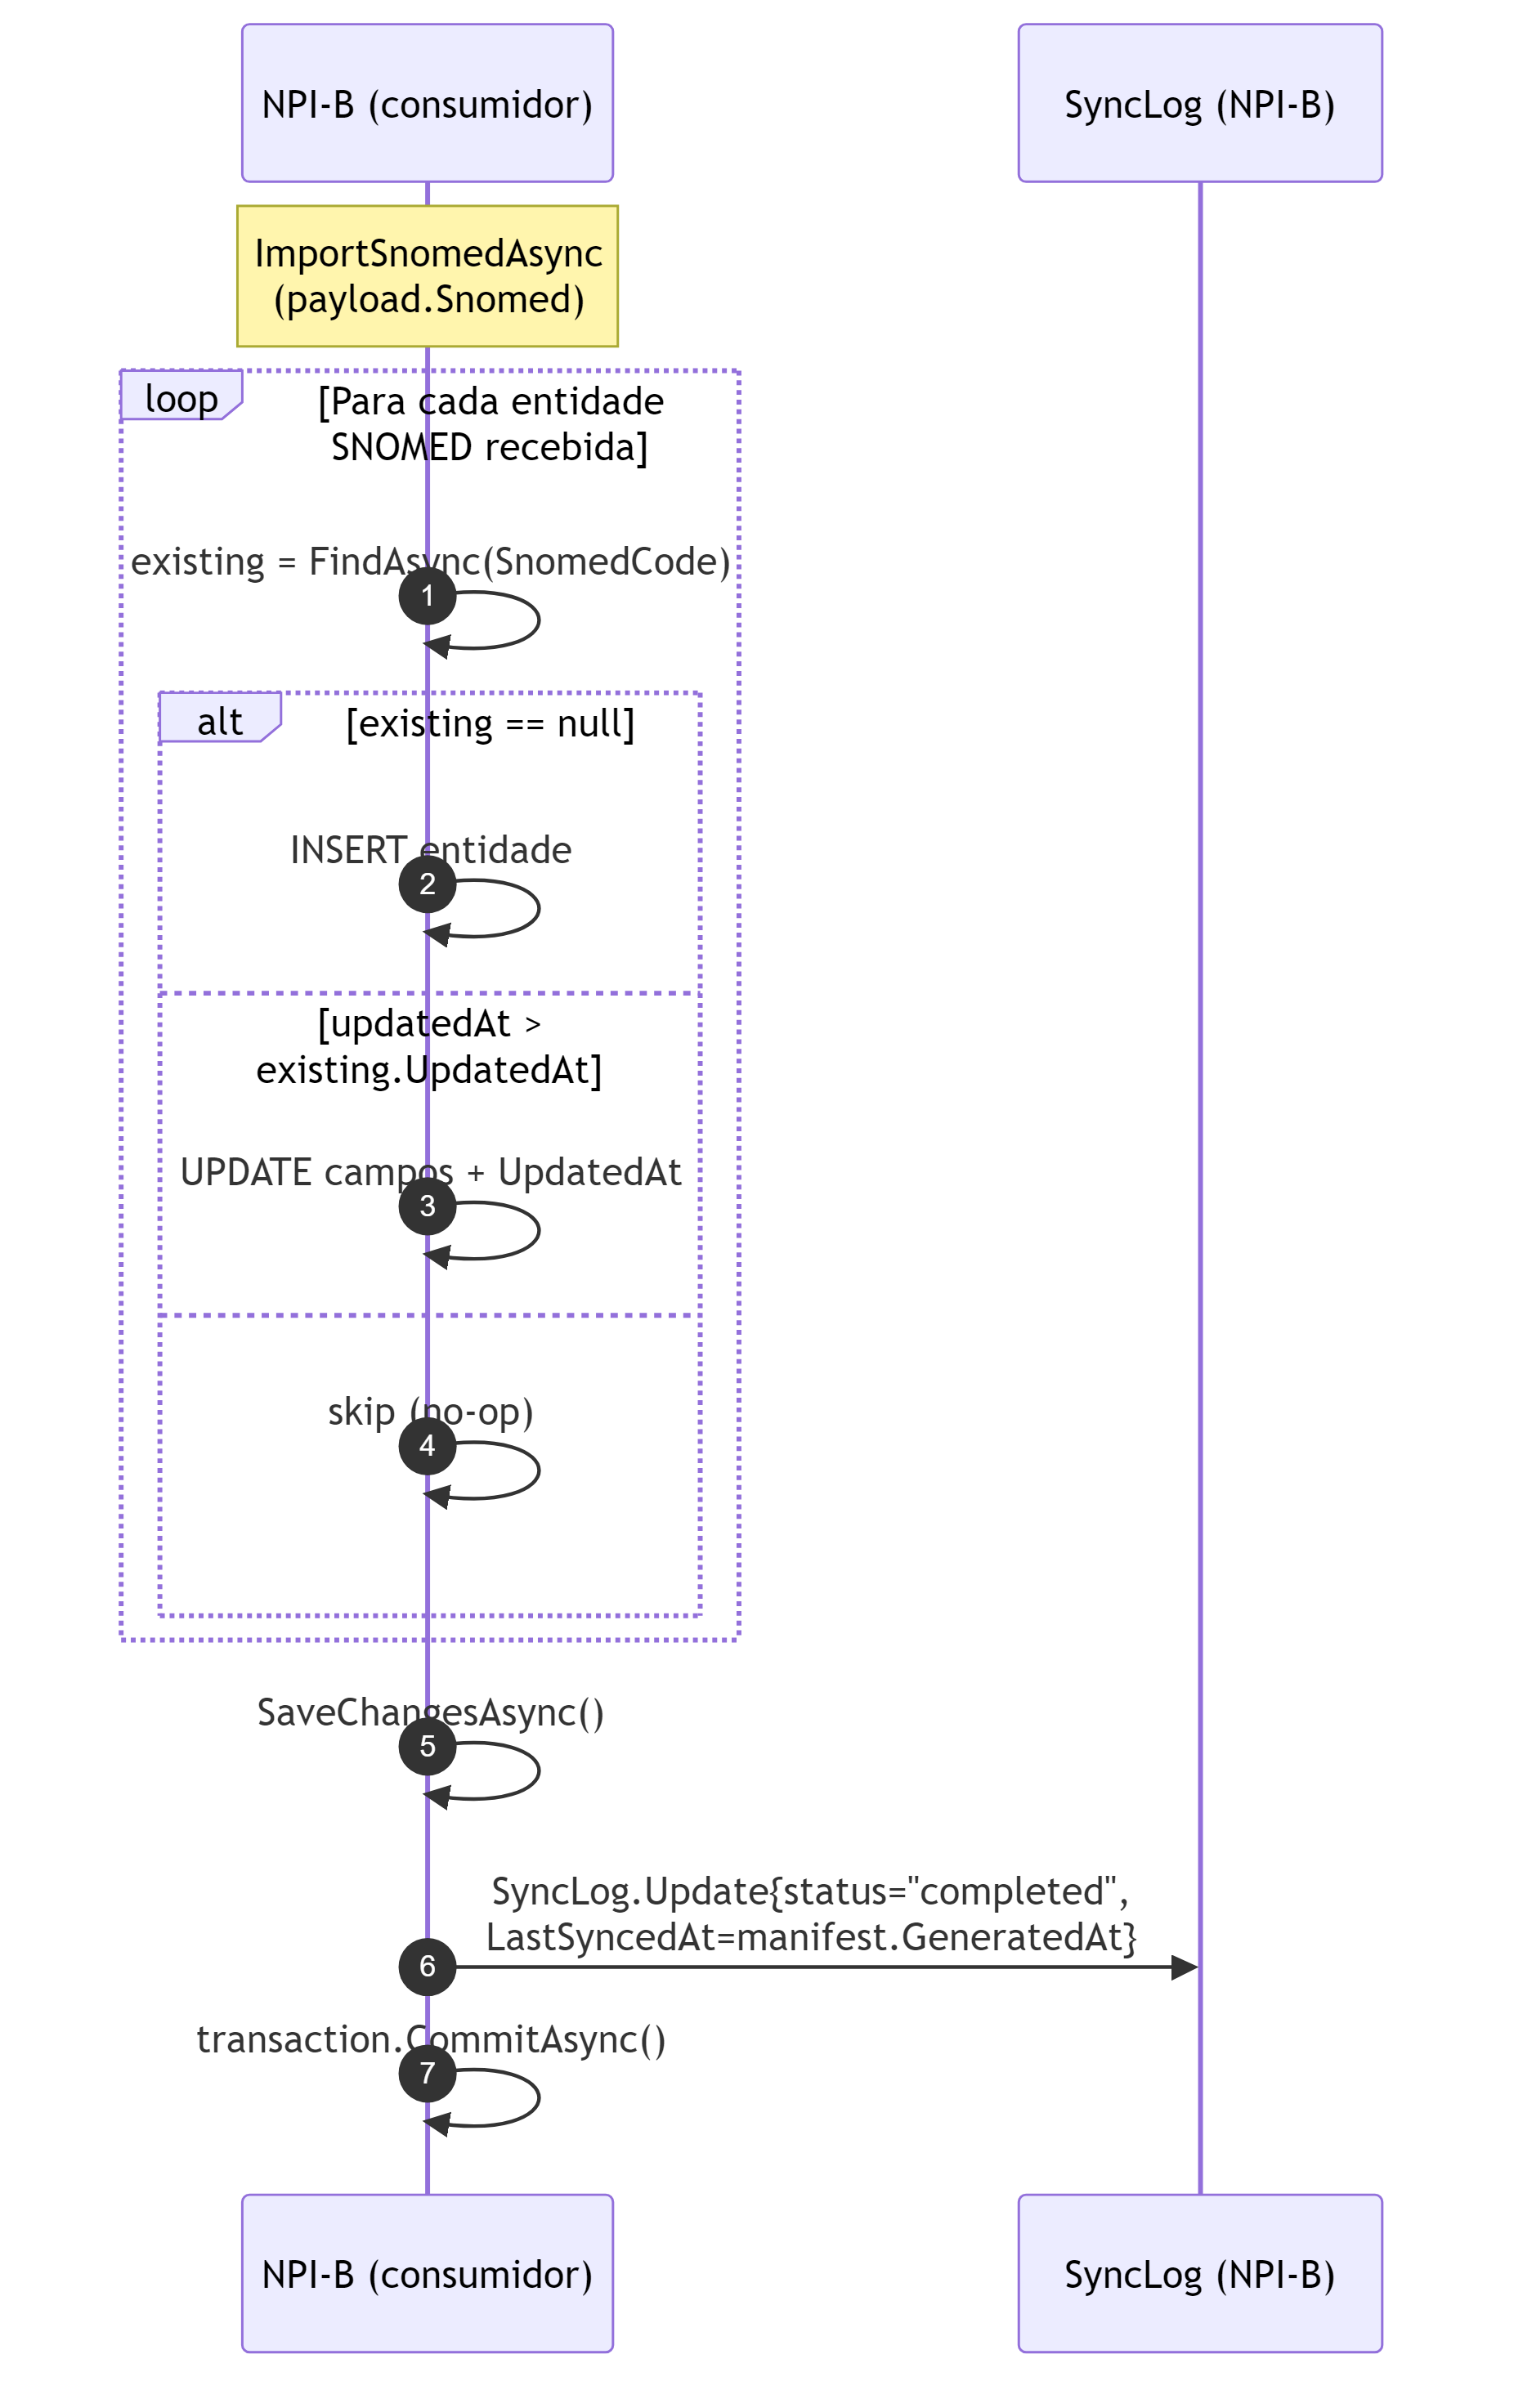
\includegraphics[scale=0.2]{figuras/Desenvolvimento/NPI/sync-catalogo-3-import.png}
\fonte{}
\end{figure}

\begin{figure}[htpb]
\caption{Transferência de biossinais --- metadados paginados de \texttt{RecordingSession}.}
\label{fig:NPISyncBiossinais}
\label{fig:NPISyncBiossinaisMetadados}
\centering
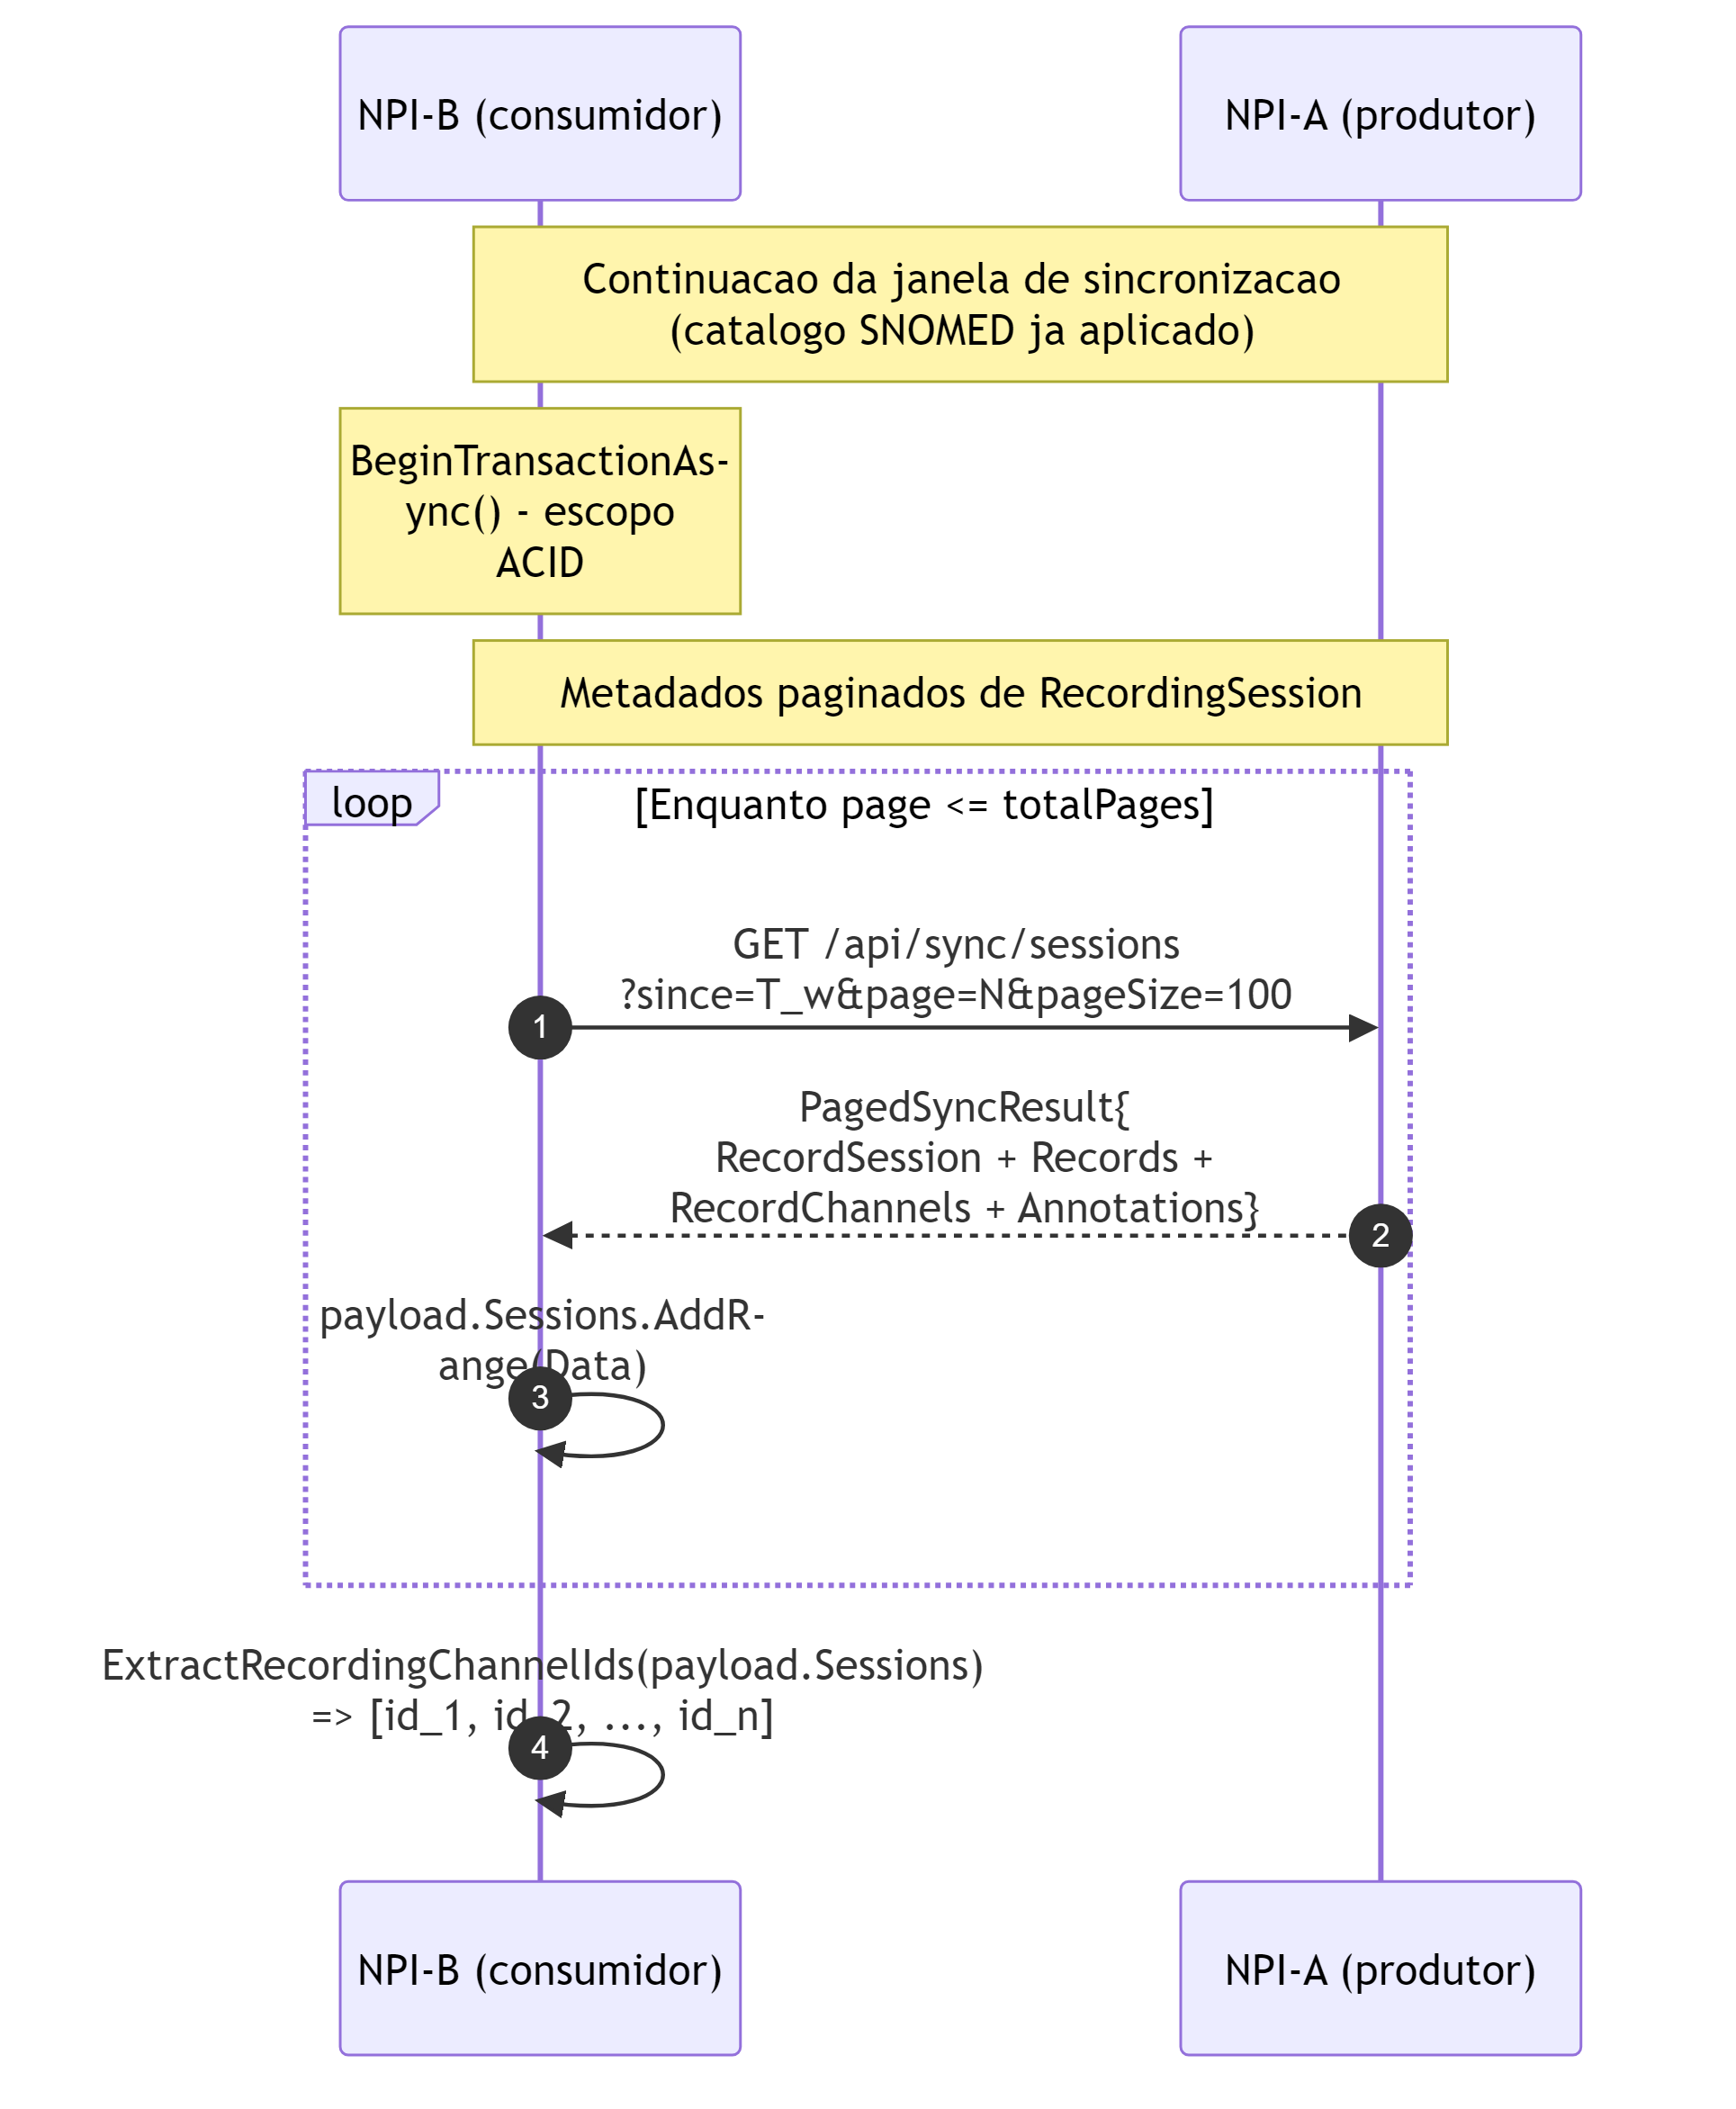
\includegraphics[width=\textwidth]{figuras/Desenvolvimento/NPI/sync-biossinais-1-metadados.png}
\fonte{}
\end{figure}

\begin{figure}[htpb]
\caption{Transferência de biossinais --- recuperação de arquivos binários por \texttt{RecordChannel} e \textit{upload} ao \textit{blob storage}.}
\label{fig:NPISyncBiossinaisBinarios}
\centering
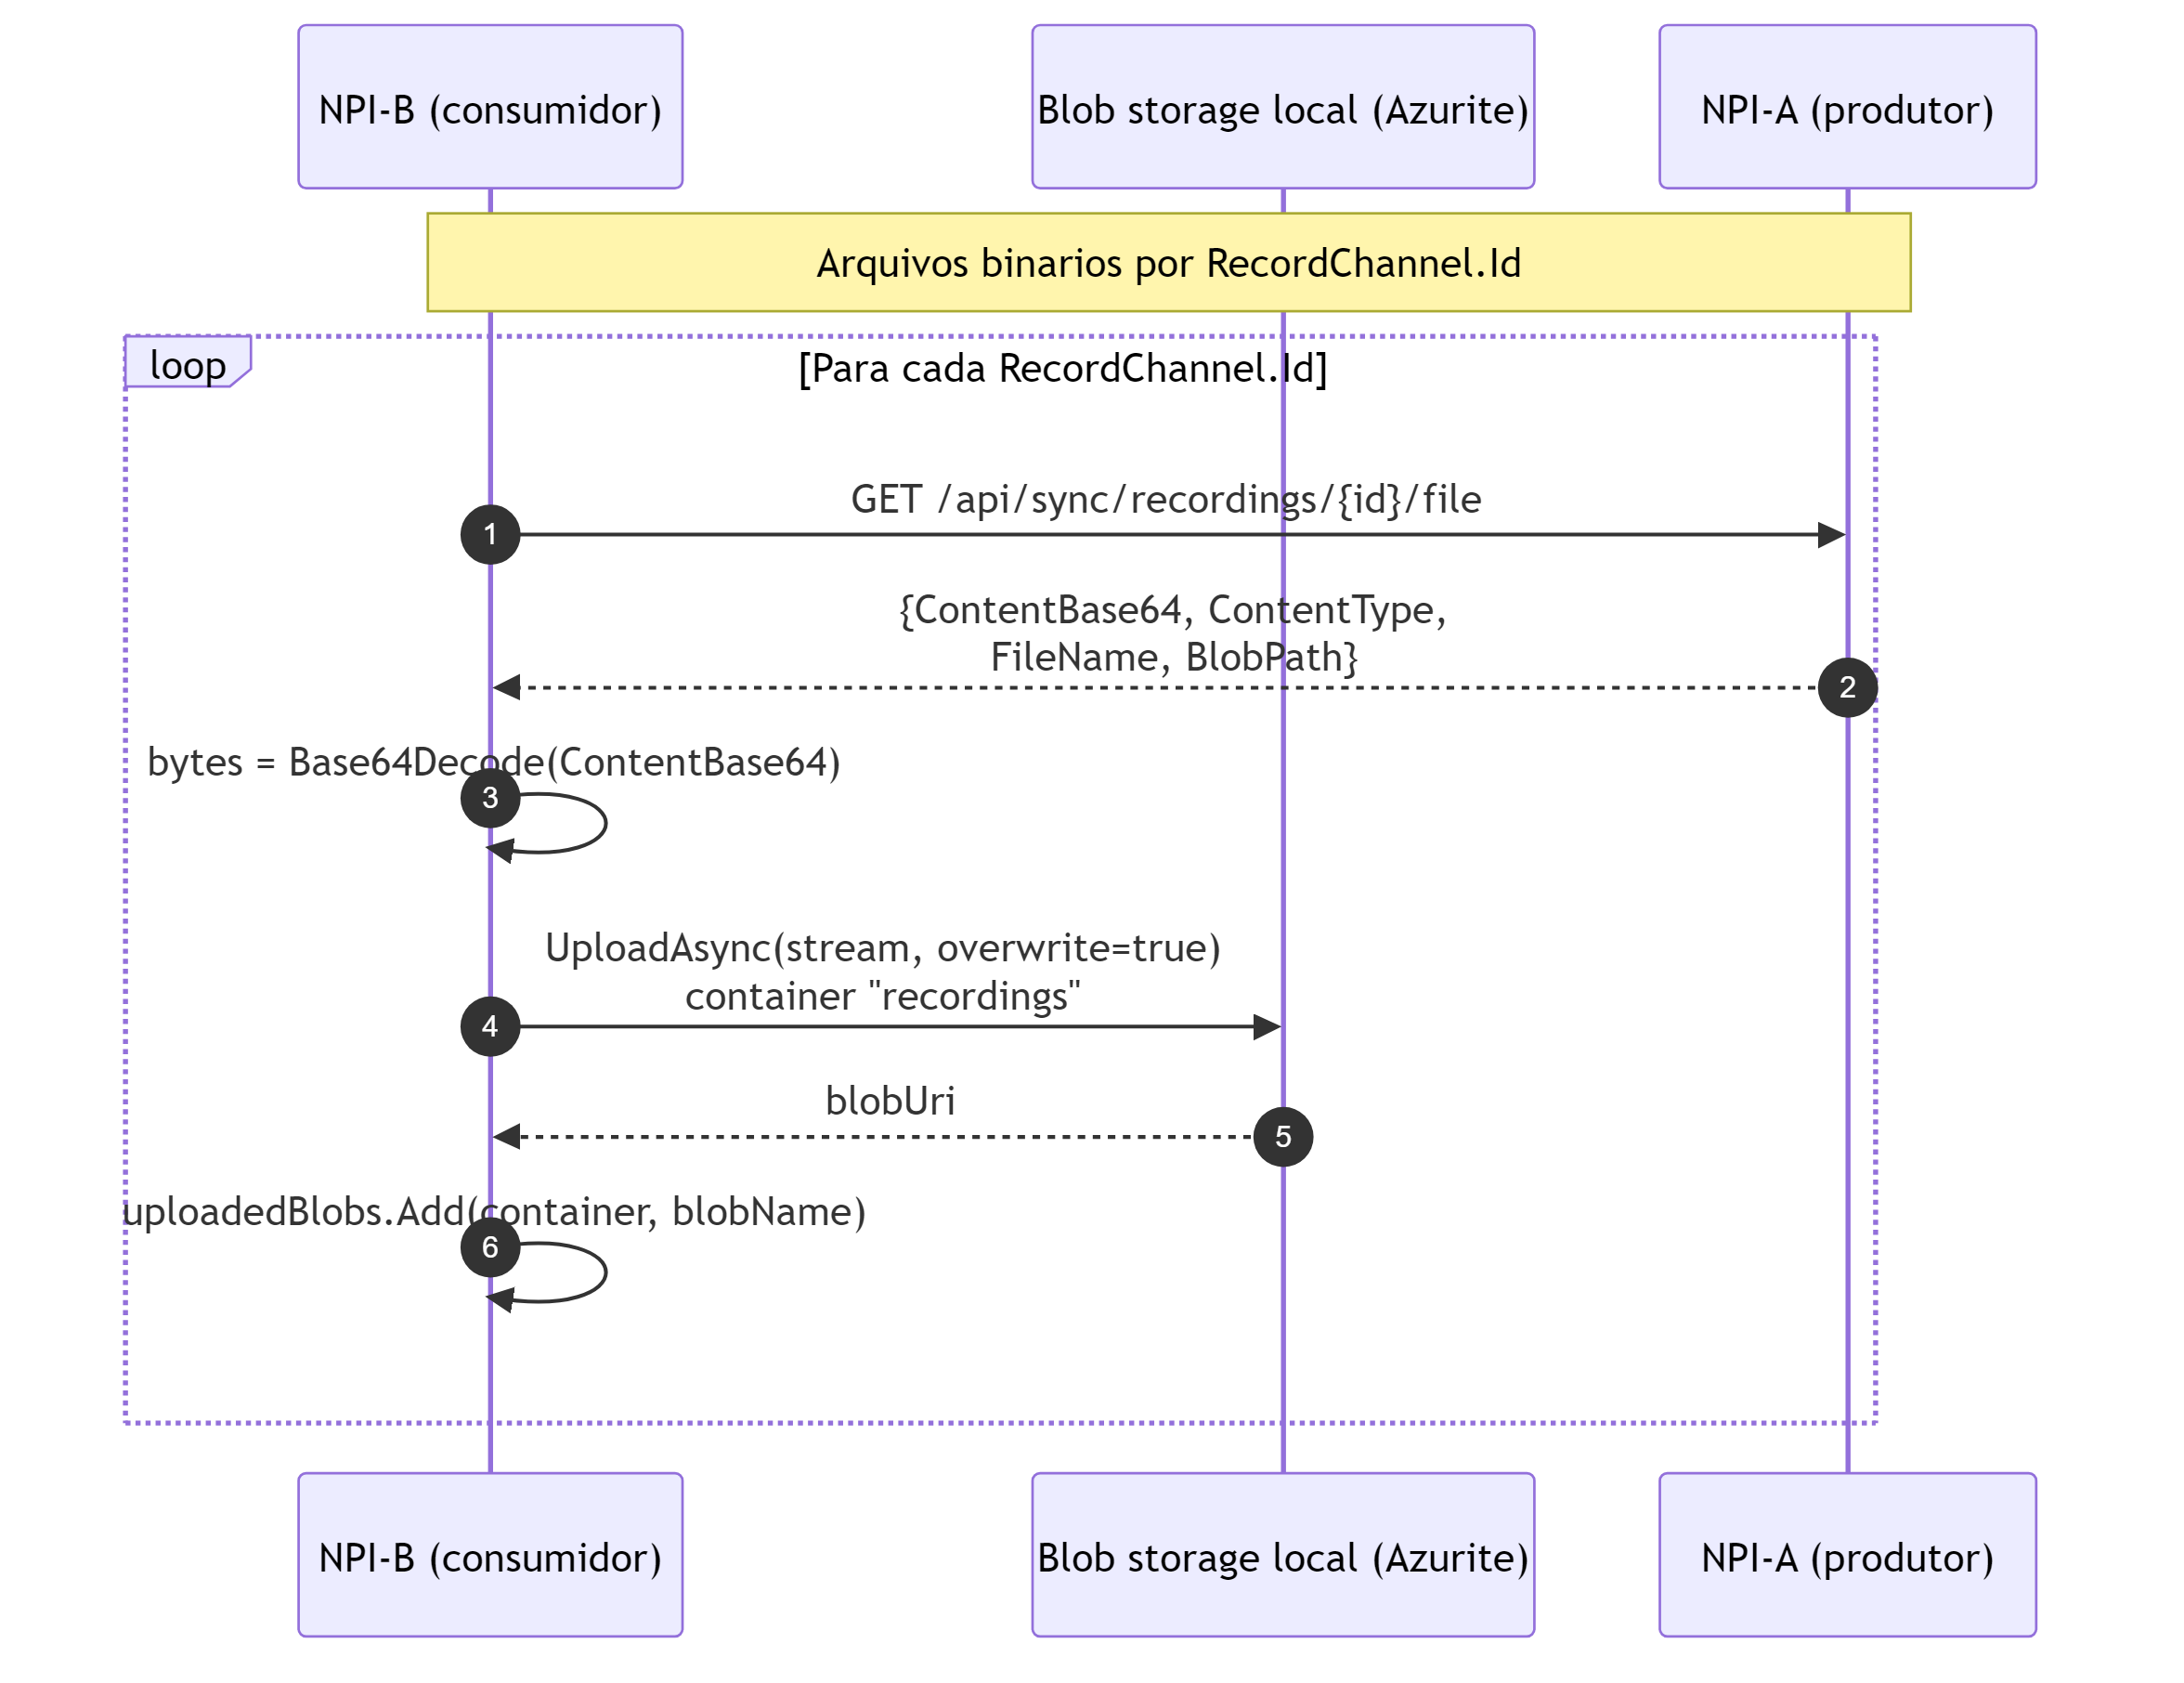
\includegraphics[width=\textwidth]{figuras/Desenvolvimento/NPI/sync-biossinais-2-binarios.png}
\fonte{}
\end{figure}

\begin{figure}[htpb]
\caption{Transferência de biossinais --- \textit{commit} transacional e ação compensatória em caso de falha.}
\label{fig:NPISyncBiossinaisCommit}
\centering
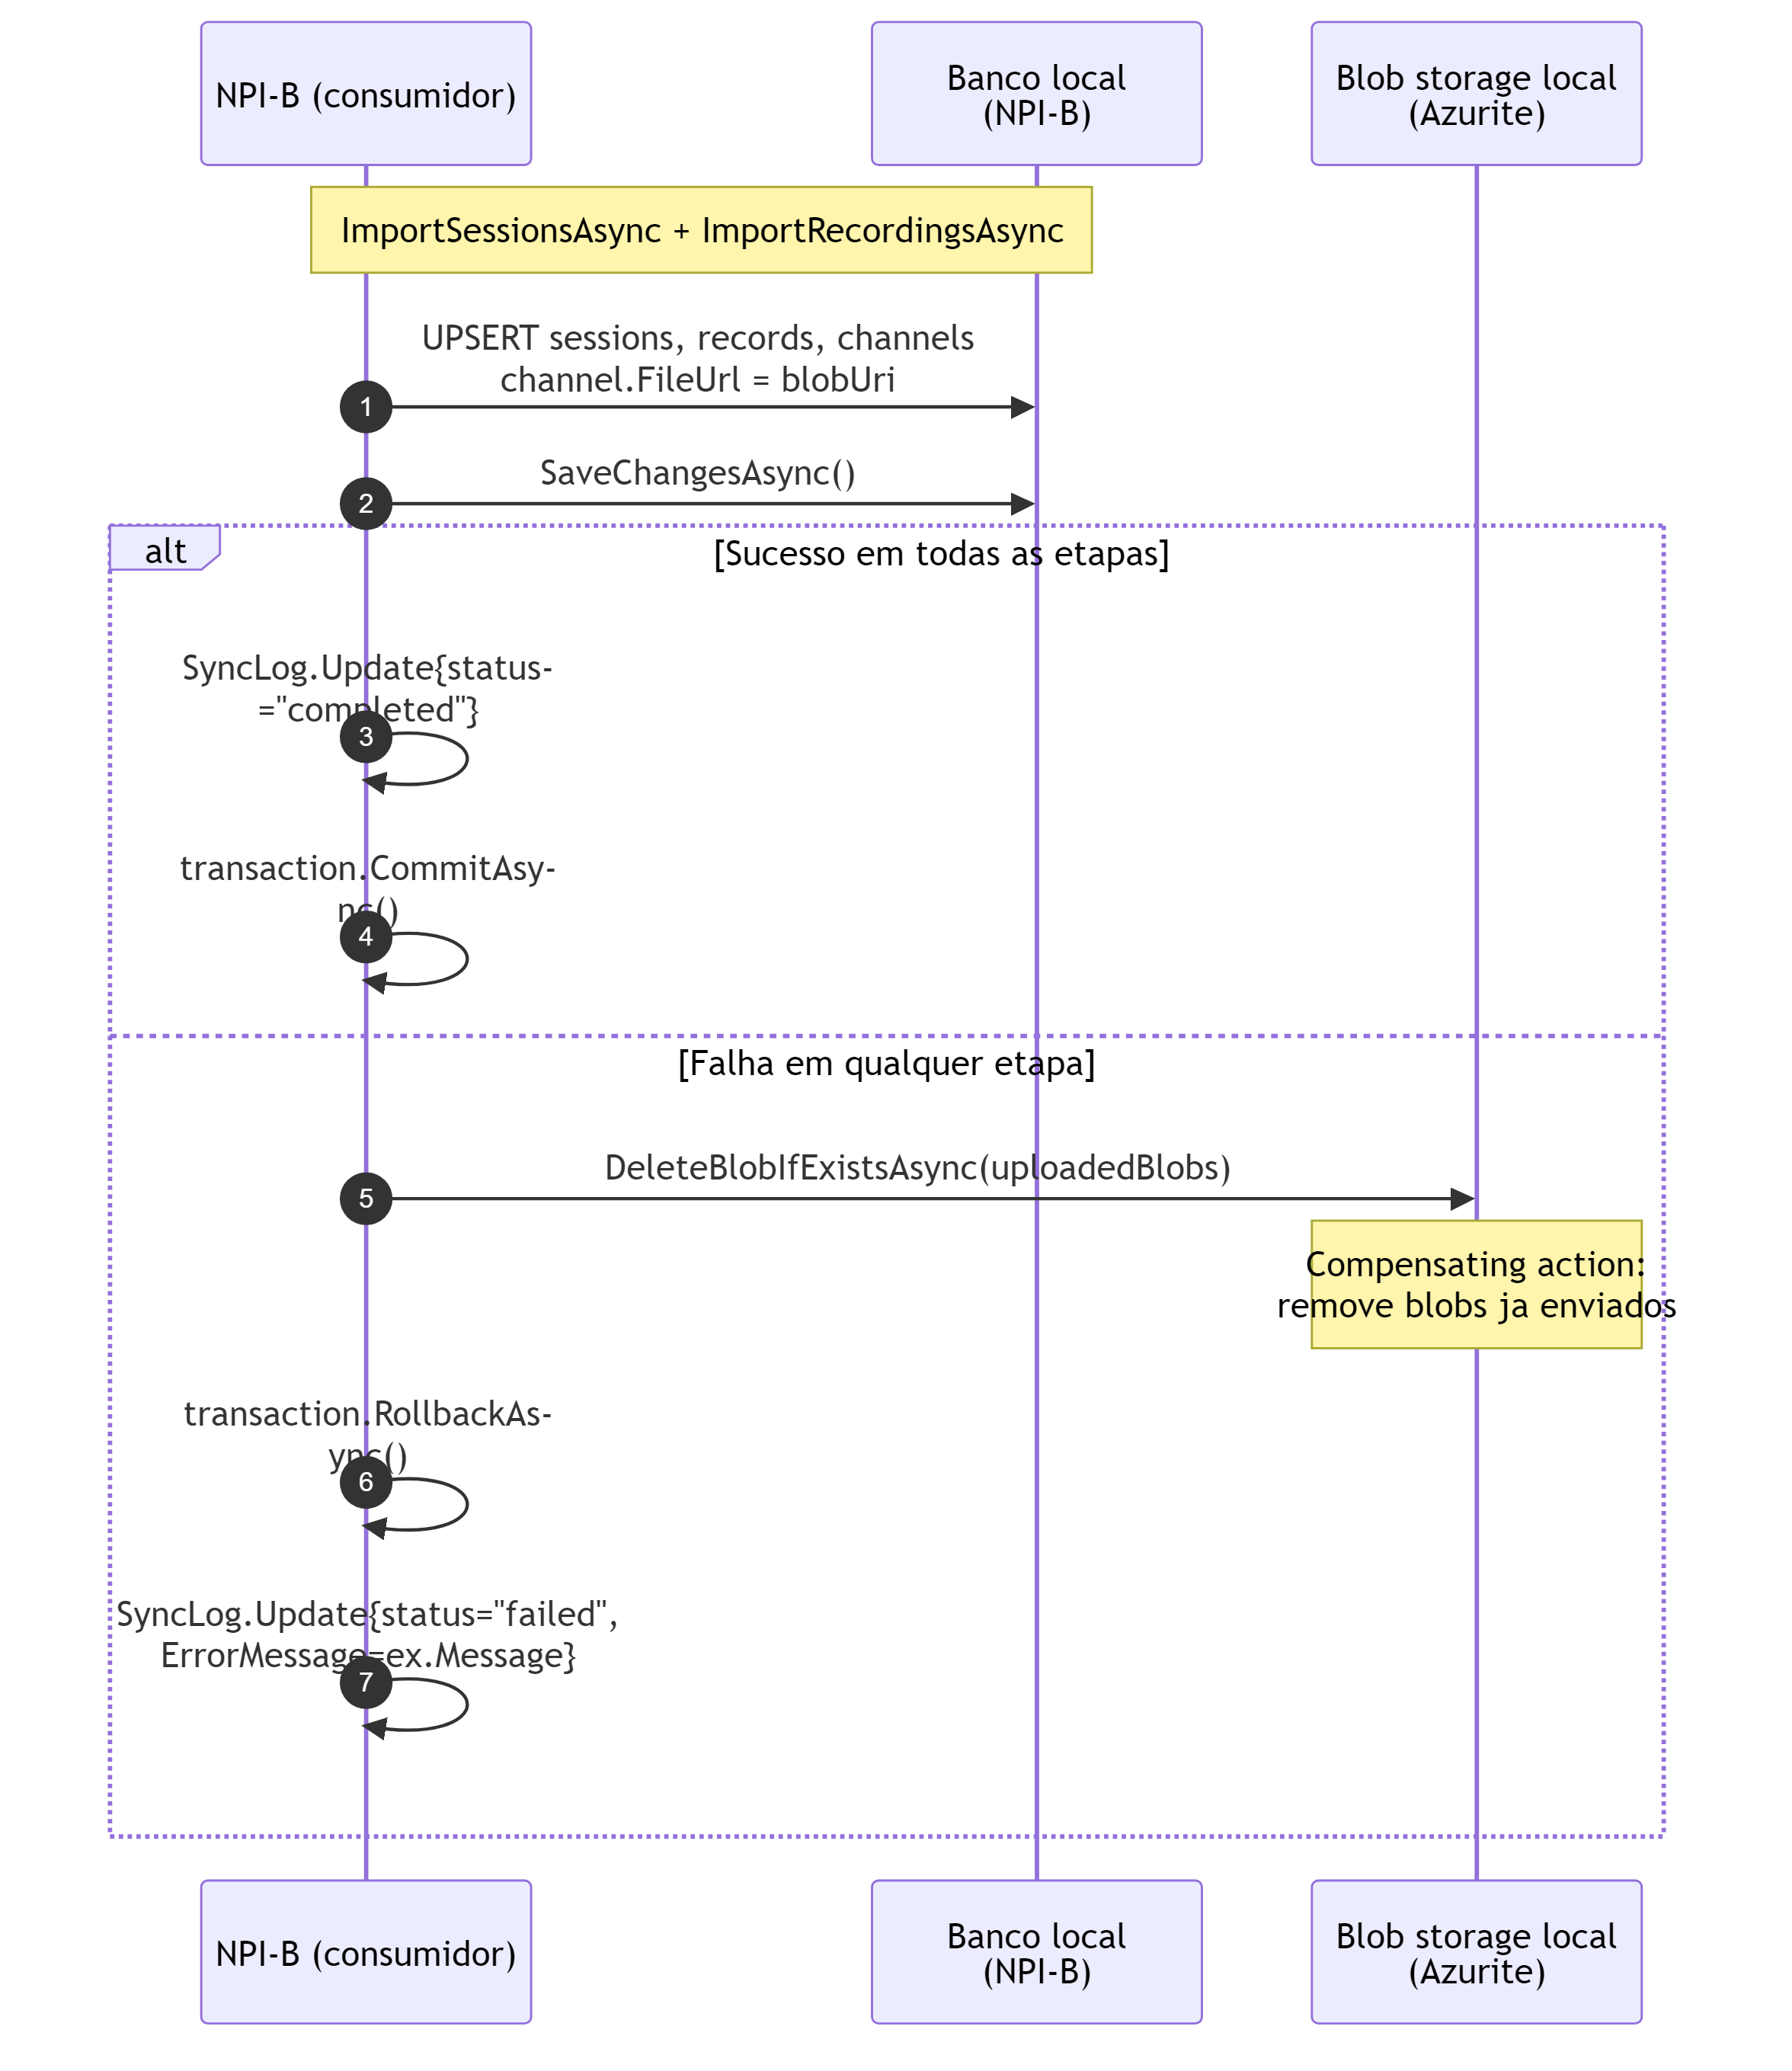
\includegraphics[width=\textwidth]{figuras/Desenvolvimento/NPI/sync-biossinais-3-commit.png}
\fonte{}
\end{figure}

\begin{figure}[htpb]
\captionsetup{width=\textwidth}
\caption{Idempotência sob retransmissão: detecção por UUID e \textit{watermark} \texttt{UpdatedAt}.}
\label{fig:NPIIdempotencia}
\centering
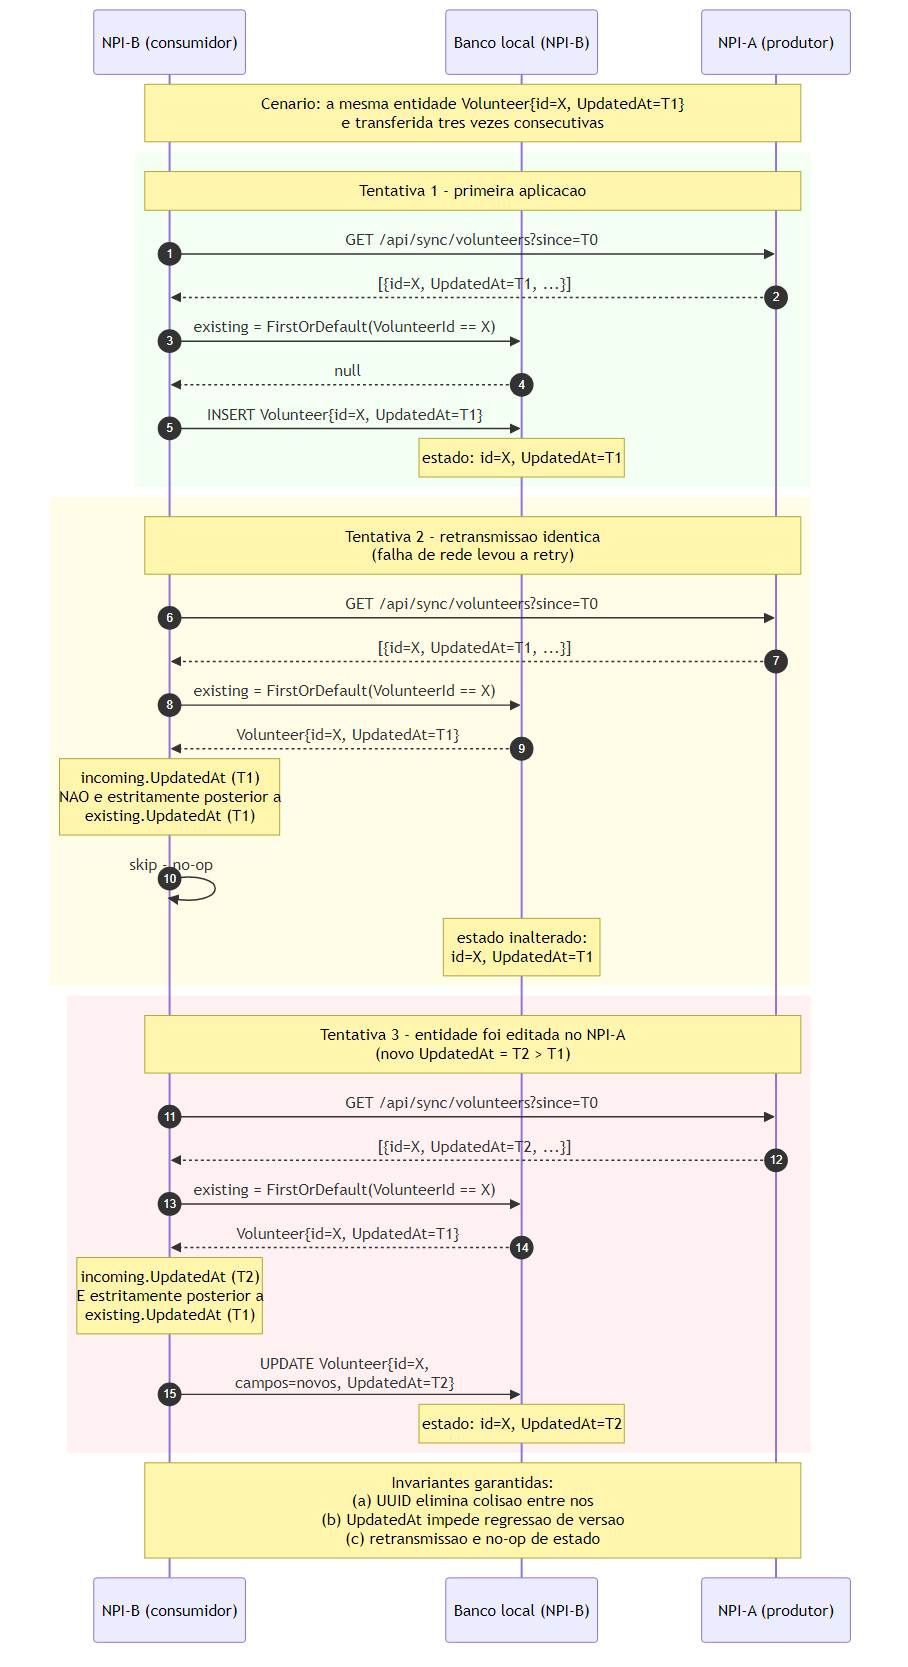
\includegraphics[scale=0.16]{figuras/Desenvolvimento/NPI/idempotencia.png}
\fonte{}
\end{figure}

% ----------------------------------------------------------------------
\section{Orquestração da federação no IRIS \emph{web}}\label{sec:apendiceSeqIRIS}
% ----------------------------------------------------------------------

Os dois diagramas desta seção complementam a discussão da Subseção~\ref{subsubsec:IRISFederacao} sobre o módulo de federação do IRIS \emph{web}. A Figura~\ref{fig:IRISEstadosConexao} apresenta a máquina de estados que rege o ciclo de vida de uma conexão federada \texttt{ResearchNodeConnection}: a transição de \texttt{UNKNOWN} para \texttt{PENDING} quando o administrador local submete a solicitação, a aprovação para \texttt{AUTHORIZED} e a possibilidade de revogação posterior para \texttt{REVOKED}, com reaprovação subsequente. A Figura~\ref{fig:IRISFluxoSync} representa o fluxo orquestrado pelo \texttt{SyncProgressModal} em conjunto com o serviço \texttt{NodeSyncServiceAdapter}, dividido em duas etapas explicitamente apresentadas ao usuário: a pré-visualização (\texttt{POST /api/sync/preview}) que retorna o manifesto das entidades disponíveis no nó remoto, e o \textit{pull} efetivo (\texttt{POST /api/sync/pull}) que dispara a transação atômica responsável pela ingestão dos dados.

\begin{figure}[htpb]
\caption{Ciclo de vida de uma conexão federada \texttt{ResearchNodeConnection} no IRIS \emph{web}.}
\label{fig:IRISEstadosConexao}
\centering
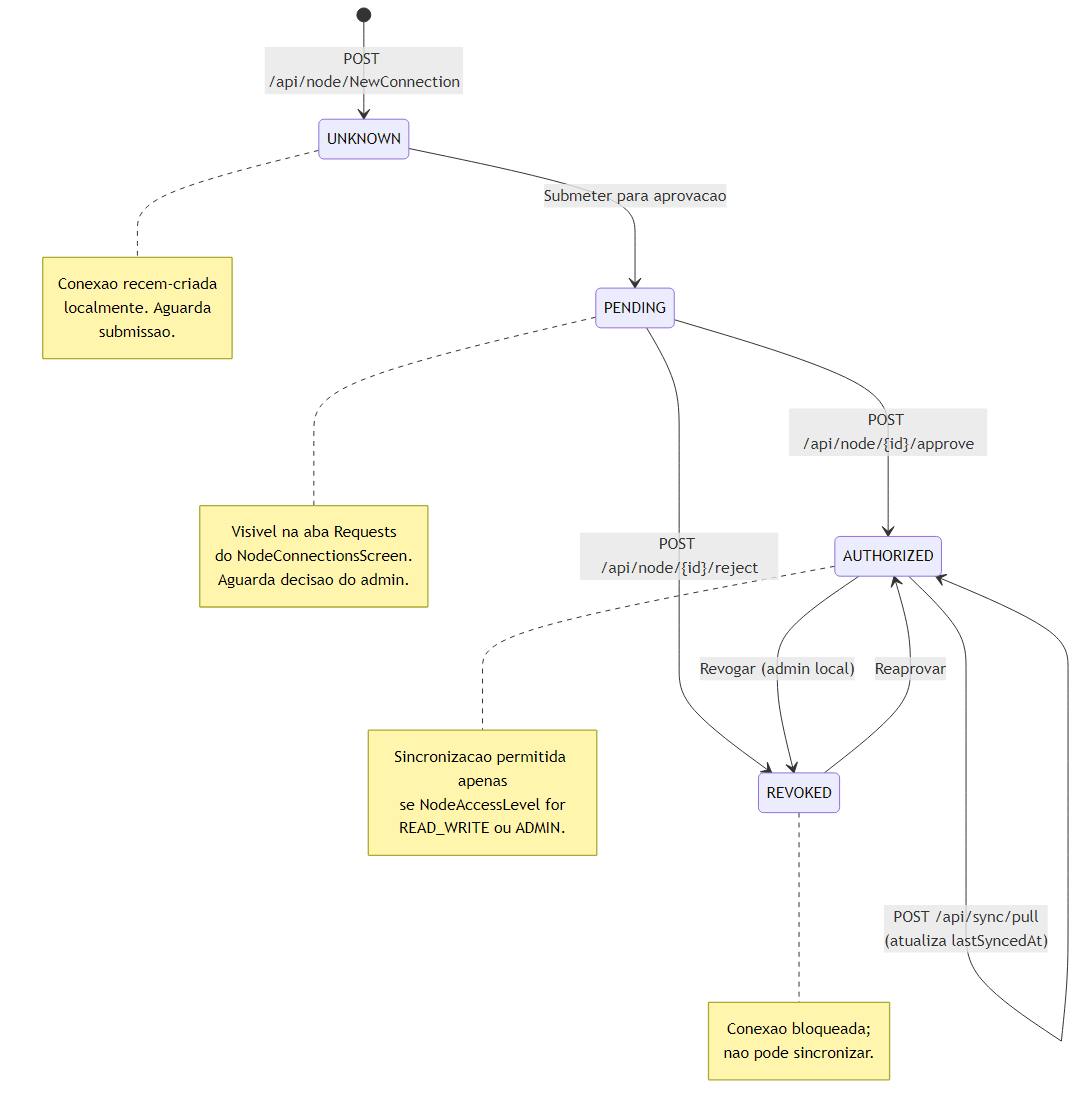
\includegraphics[scale=0.5]{figuras/Desenvolvimento/IRIS/estados-conexao-npi.png}
\fonte{}
\end{figure}

\begin{figure}[htpb]
\caption{Fluxo de sincronização de dados entre NPIs orquestrado pelo IRIS \emph{web}.}
\label{fig:IRISFluxoSync}
\centering
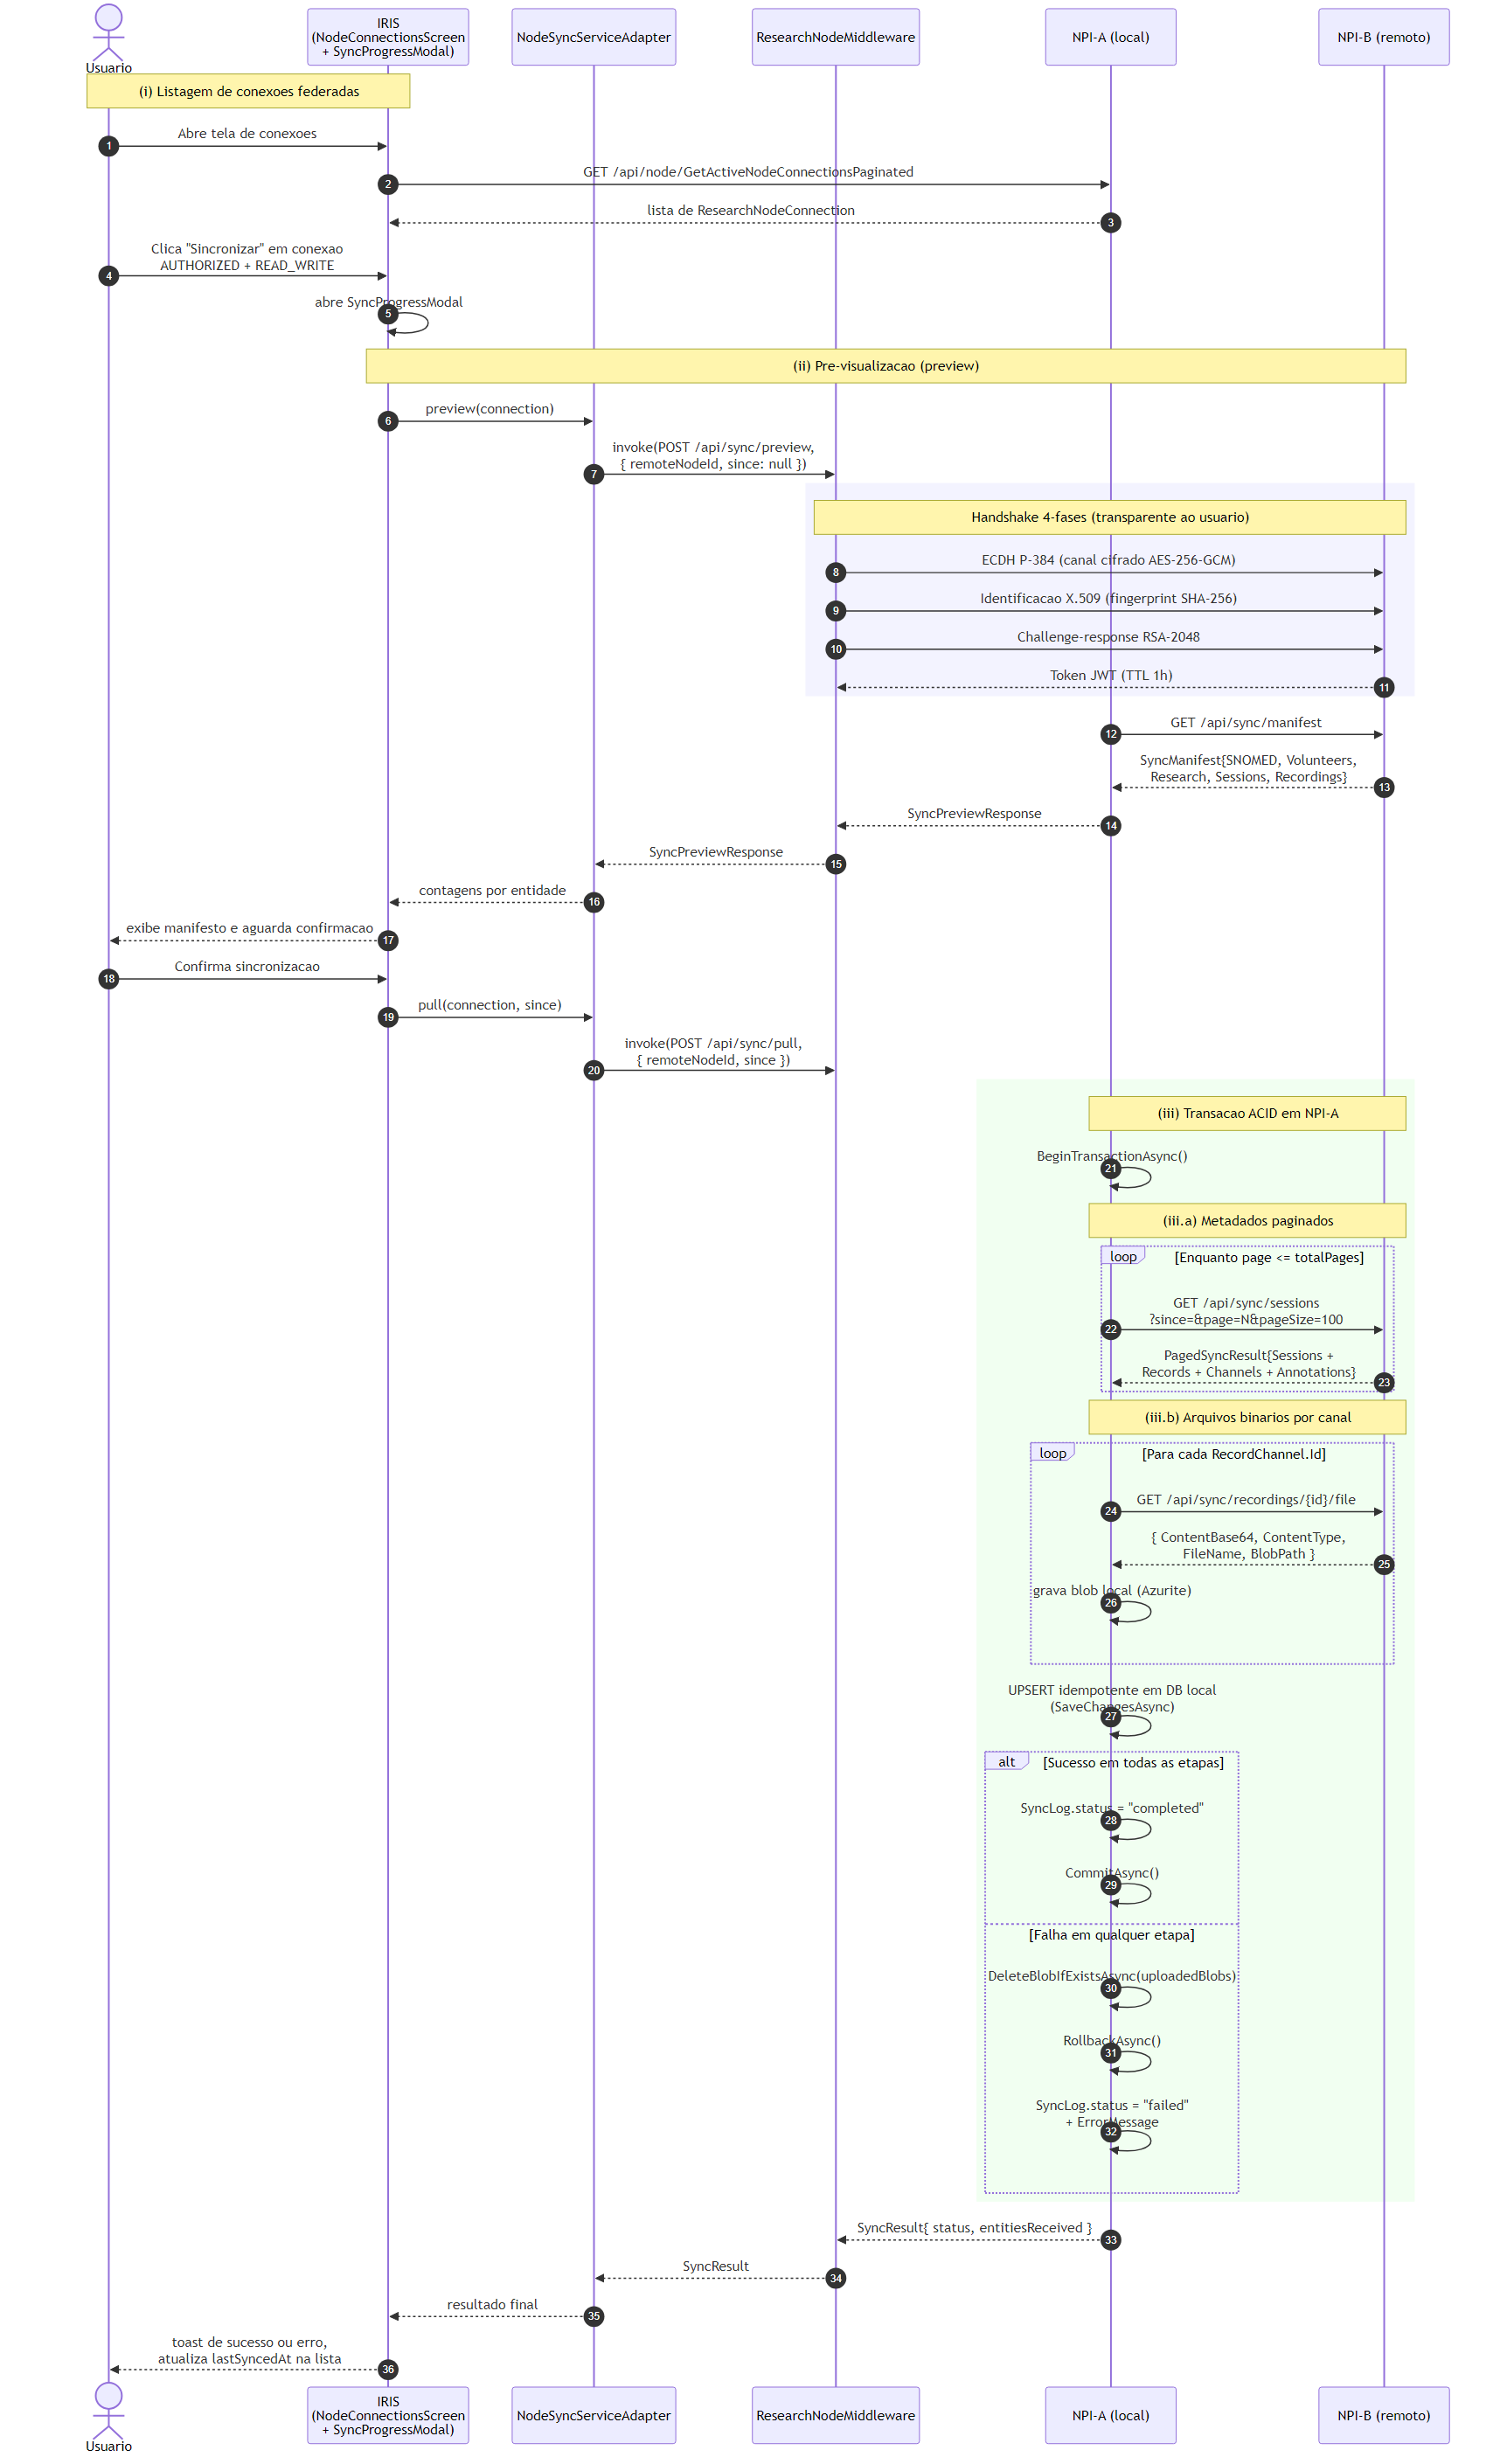
\includegraphics[scale=0.3, angle=90]{figuras/Desenvolvimento/IRIS/fluxo-sincronizacao-iris.png}
\fonte{}
\end{figure}

% ----------------------------------------------------------------------
\section{Fluxos do IRIS \textit{Mobile}}\label{sec:apendiceSeqMobile}
% ----------------------------------------------------------------------

Esta seção reúne os oito diagramas que detalham os três fluxos centrais do IRIS \textit{Mobile}, em correspondência com as Subseções~\ref{subsec:IRISMobileBT}, \ref{subsec:IRISMobileCaptura} e \ref{subsec:IRISMobileRotulos}. À semelhança do que ocorreu com os fluxos de sincronização entre nós (Seção~\ref{sec:apendiceSeqSync}), a extensão do diálogo entre o aplicativo, o dispositivo e o NPI tornou inviável a representação de cada fluxo em um único diagrama, e a decomposição em etapas privilegia a legibilidade individual sem sacrificar a representação completa do protocolo.

O fluxo de captura via Bluetooth é apresentado em três etapas. A Figura~\ref{fig:IRISMobileFluxoCapturaPareamento} ilustra o pareamento Bluetooth e a abertura do canal \textit{Serial Port Profile} (SPP) com o NeuroEstimulator, incluindo a solicitação de permissões nativas do Android e o registro dos \textit{listeners} de dados recebidos e de desconexão. A Figura~\ref{fig:IRISMobileFluxoCapturaStream} apresenta o regime estacionário de captura e \textit{streaming} a 215~Hz, evidenciando o papel do decodificador binário \texttt{BinaryFrameAccumulator} e a renderização decimada do sinal sEMG na \texttt{CaptureScreen}. A Figura~\ref{fig:IRISMobileFluxoCapturaEncerramento} fecha o ciclo com o encerramento ordenado da captura --- comando de \textit{stop streaming} e \textit{flush} do \textit{buffer} de CSV --- e descreve o ramo alternativo de recuperação acionado em caso de desconexão Bluetooth inesperada.

O fluxo de sincronização com o NPI é apresentado em três etapas que separam a fase \textit{offline-first} do envio assíncrono e do tratamento de seu resultado. A Figura~\ref{fig:IRISMobileFluxoSyncGeracao} mostra a geração local da sessão clínica, da gravação e das anotações em modo \textit{offline-first}, com persistência em SQLite e marcação de \texttt{sync\_status = 'pending'}. A Figura~\ref{fig:IRISMobileFluxoSyncUpload} sintetiza o ciclo periódico do \texttt{SyncService}, que percorre as três tabelas pendentes respeitando a ordem de dependências do contrato do NPI --- sessão clínica, gravação (metadados e arquivo binário) e anotações. A Figura~\ref{fig:IRISMobileFluxoSyncResultado} fecha o ciclo apresentando o tratamento do resultado da sincronização, incluindo a transição de \texttt{sync\_status} para \texttt{'synced'} ou \texttt{'failed'} e a atualização do \textit{badge} colorido exibido na \texttt{HistoryScreen}.

O fluxo de etiquetagem em tempo real é apresentado em duas etapas. A Figura~\ref{fig:IRISMobileFluxoRotulagemCriacao} percorre a criação local da anotação clínica pelo pesquisador, sua persistência em SQLite com \texttt{sync\_status = 'pending'} e o vínculo à sessão clínica em curso por meio da chave estrangeira \texttt{session\_id}. A Figura~\ref{fig:IRISMobileFluxoRotulagemEnvio} apresenta o envio assíncrono das anotações ao NPI pelo \texttt{SyncService}, condicionado à prévia sincronização da sessão à qual elas pertencem, política que preserva a integridade referencial sem necessidade de mensagens de coordenação adicionais.

\begin{figure}[htpb]
\caption{IRIS \textit{Mobile} --- pareamento Bluetooth e abertura do canal SPP com o NeuroEstimulator.}
\label{fig:IRISMobileFluxoCaptura}
\label{fig:IRISMobileFluxoCapturaPareamento}
\centering
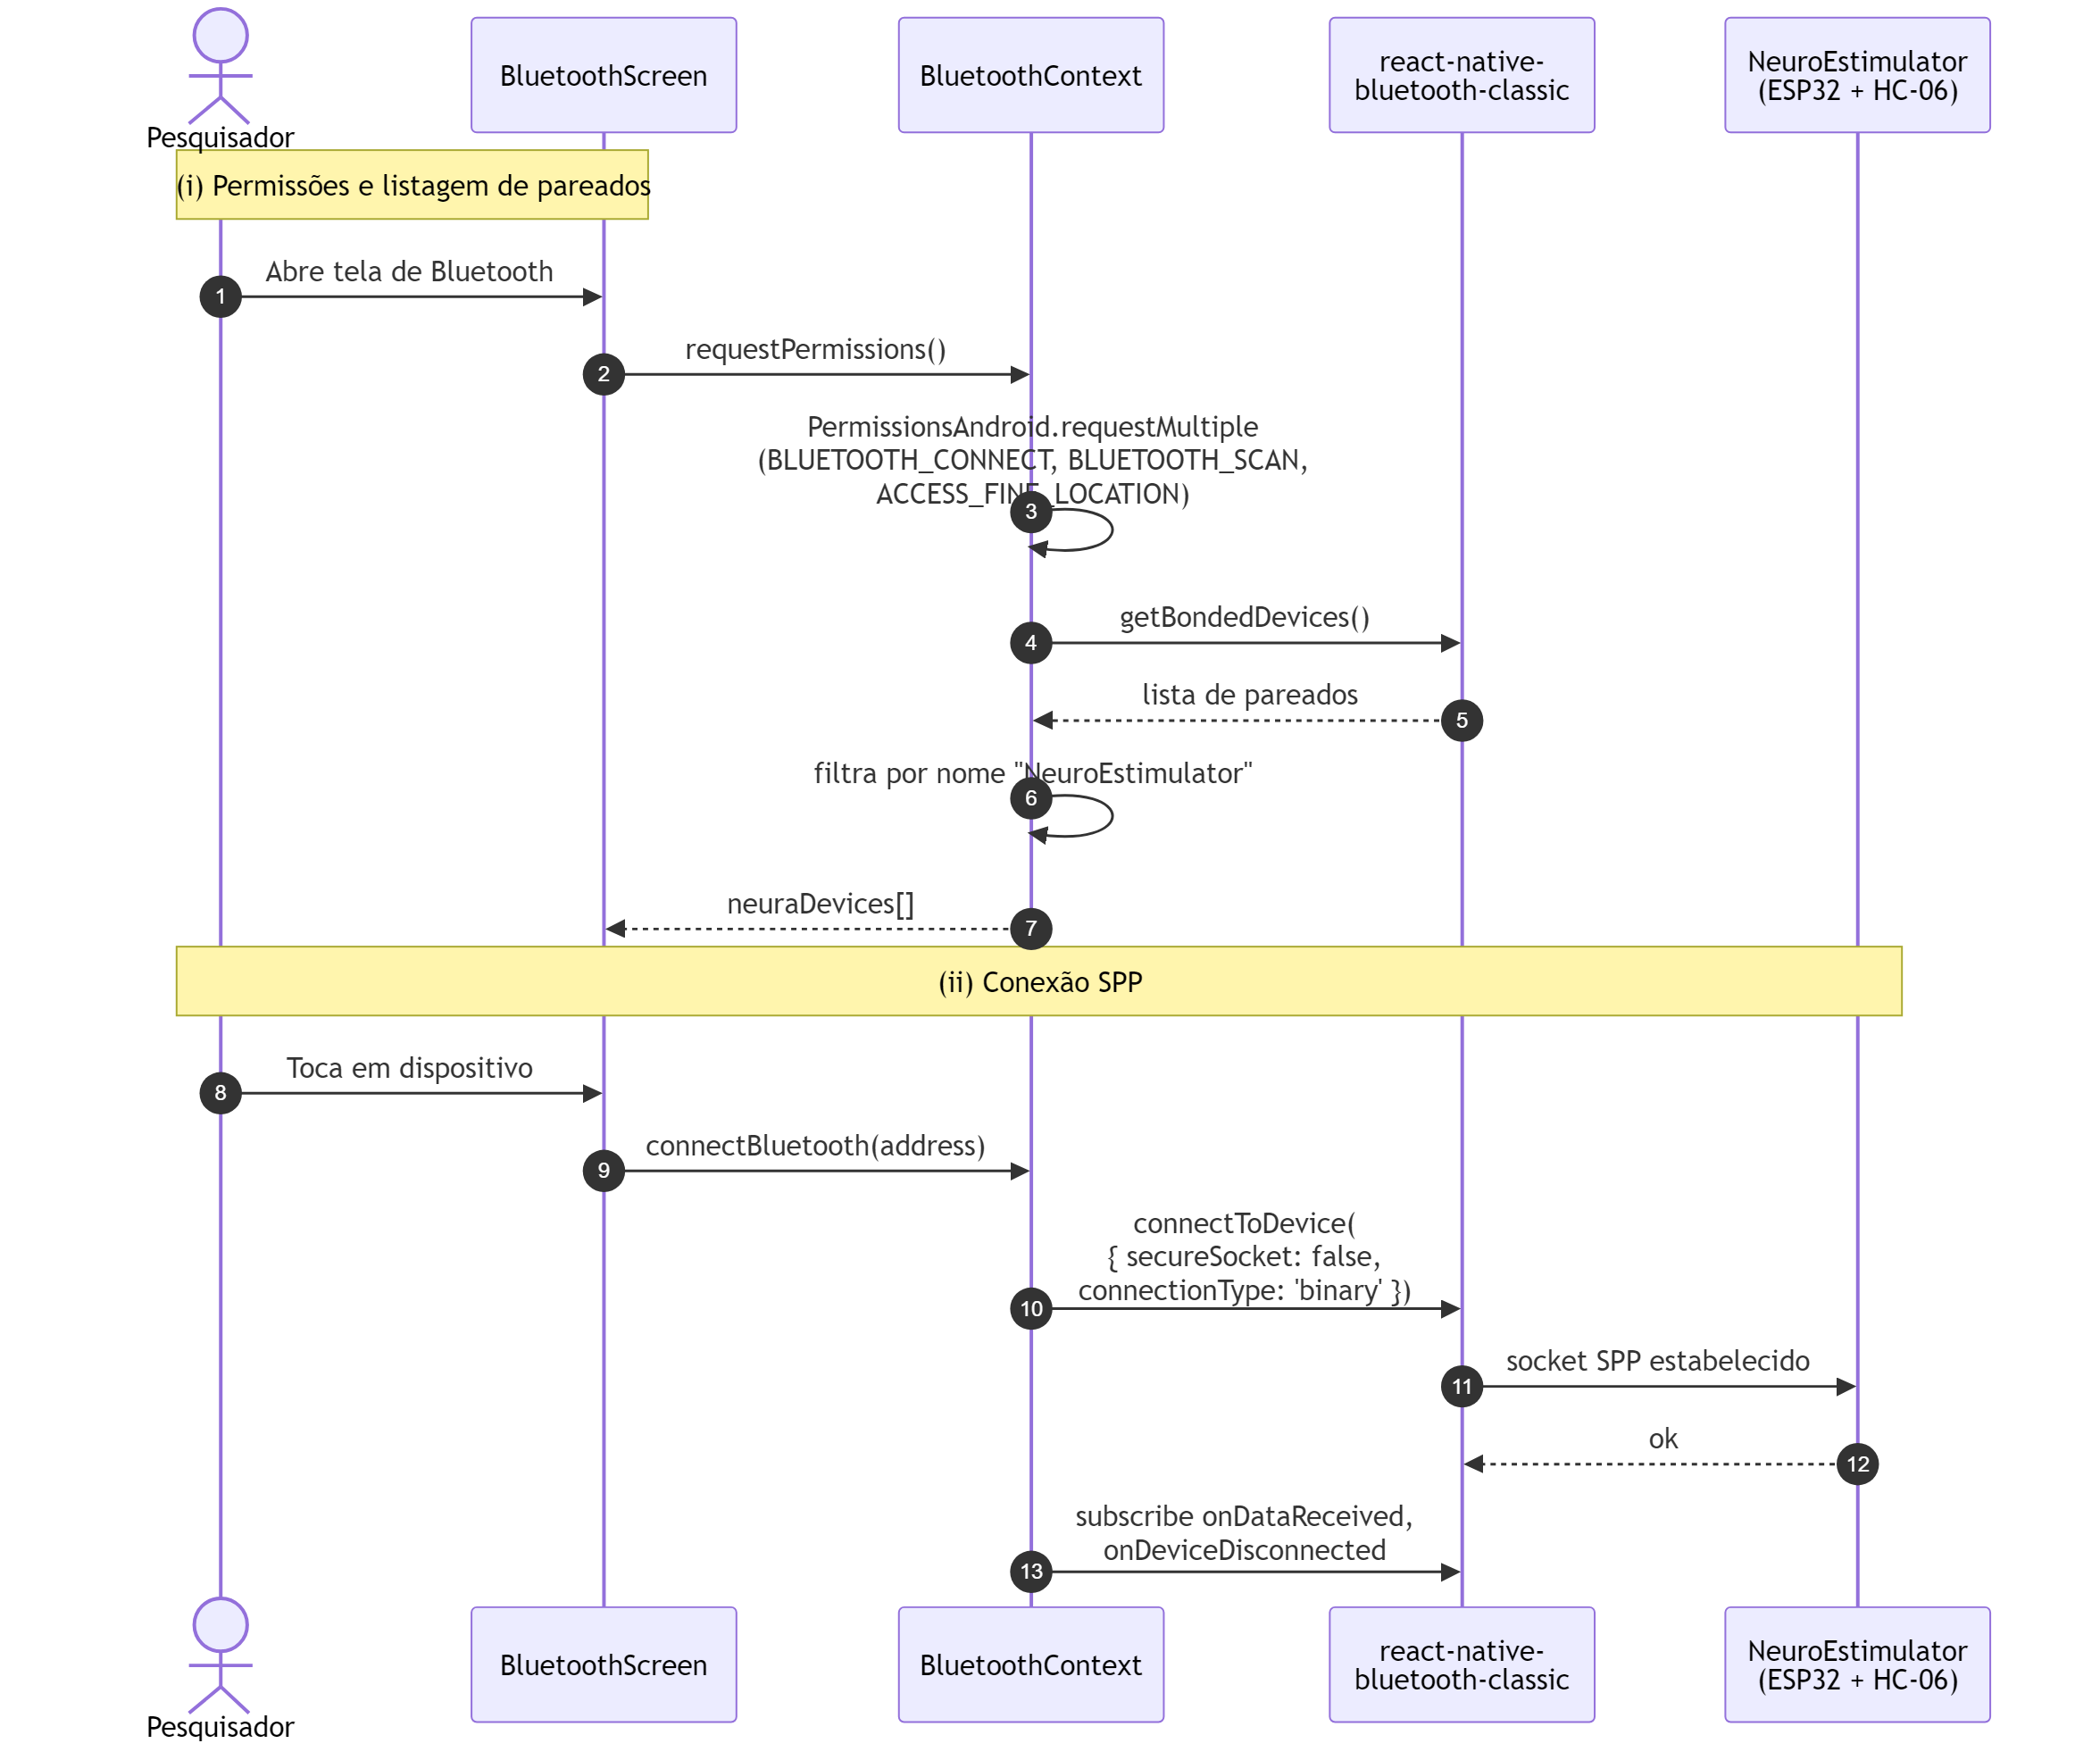
\includegraphics[scale=0.5]{figuras/Desenvolvimento/IRISMobile/fluxo-bt-streaming-1-pareamento.png}
\fonte{}
\end{figure}

\begin{figure}[htpb]
\caption{IRIS \textit{Mobile} --- captura e \textit{streaming} a 215~Hz, com decodificação binária e renderização do sinal sEMG.}
\label{fig:IRISMobileFluxoCapturaStream}
\centering
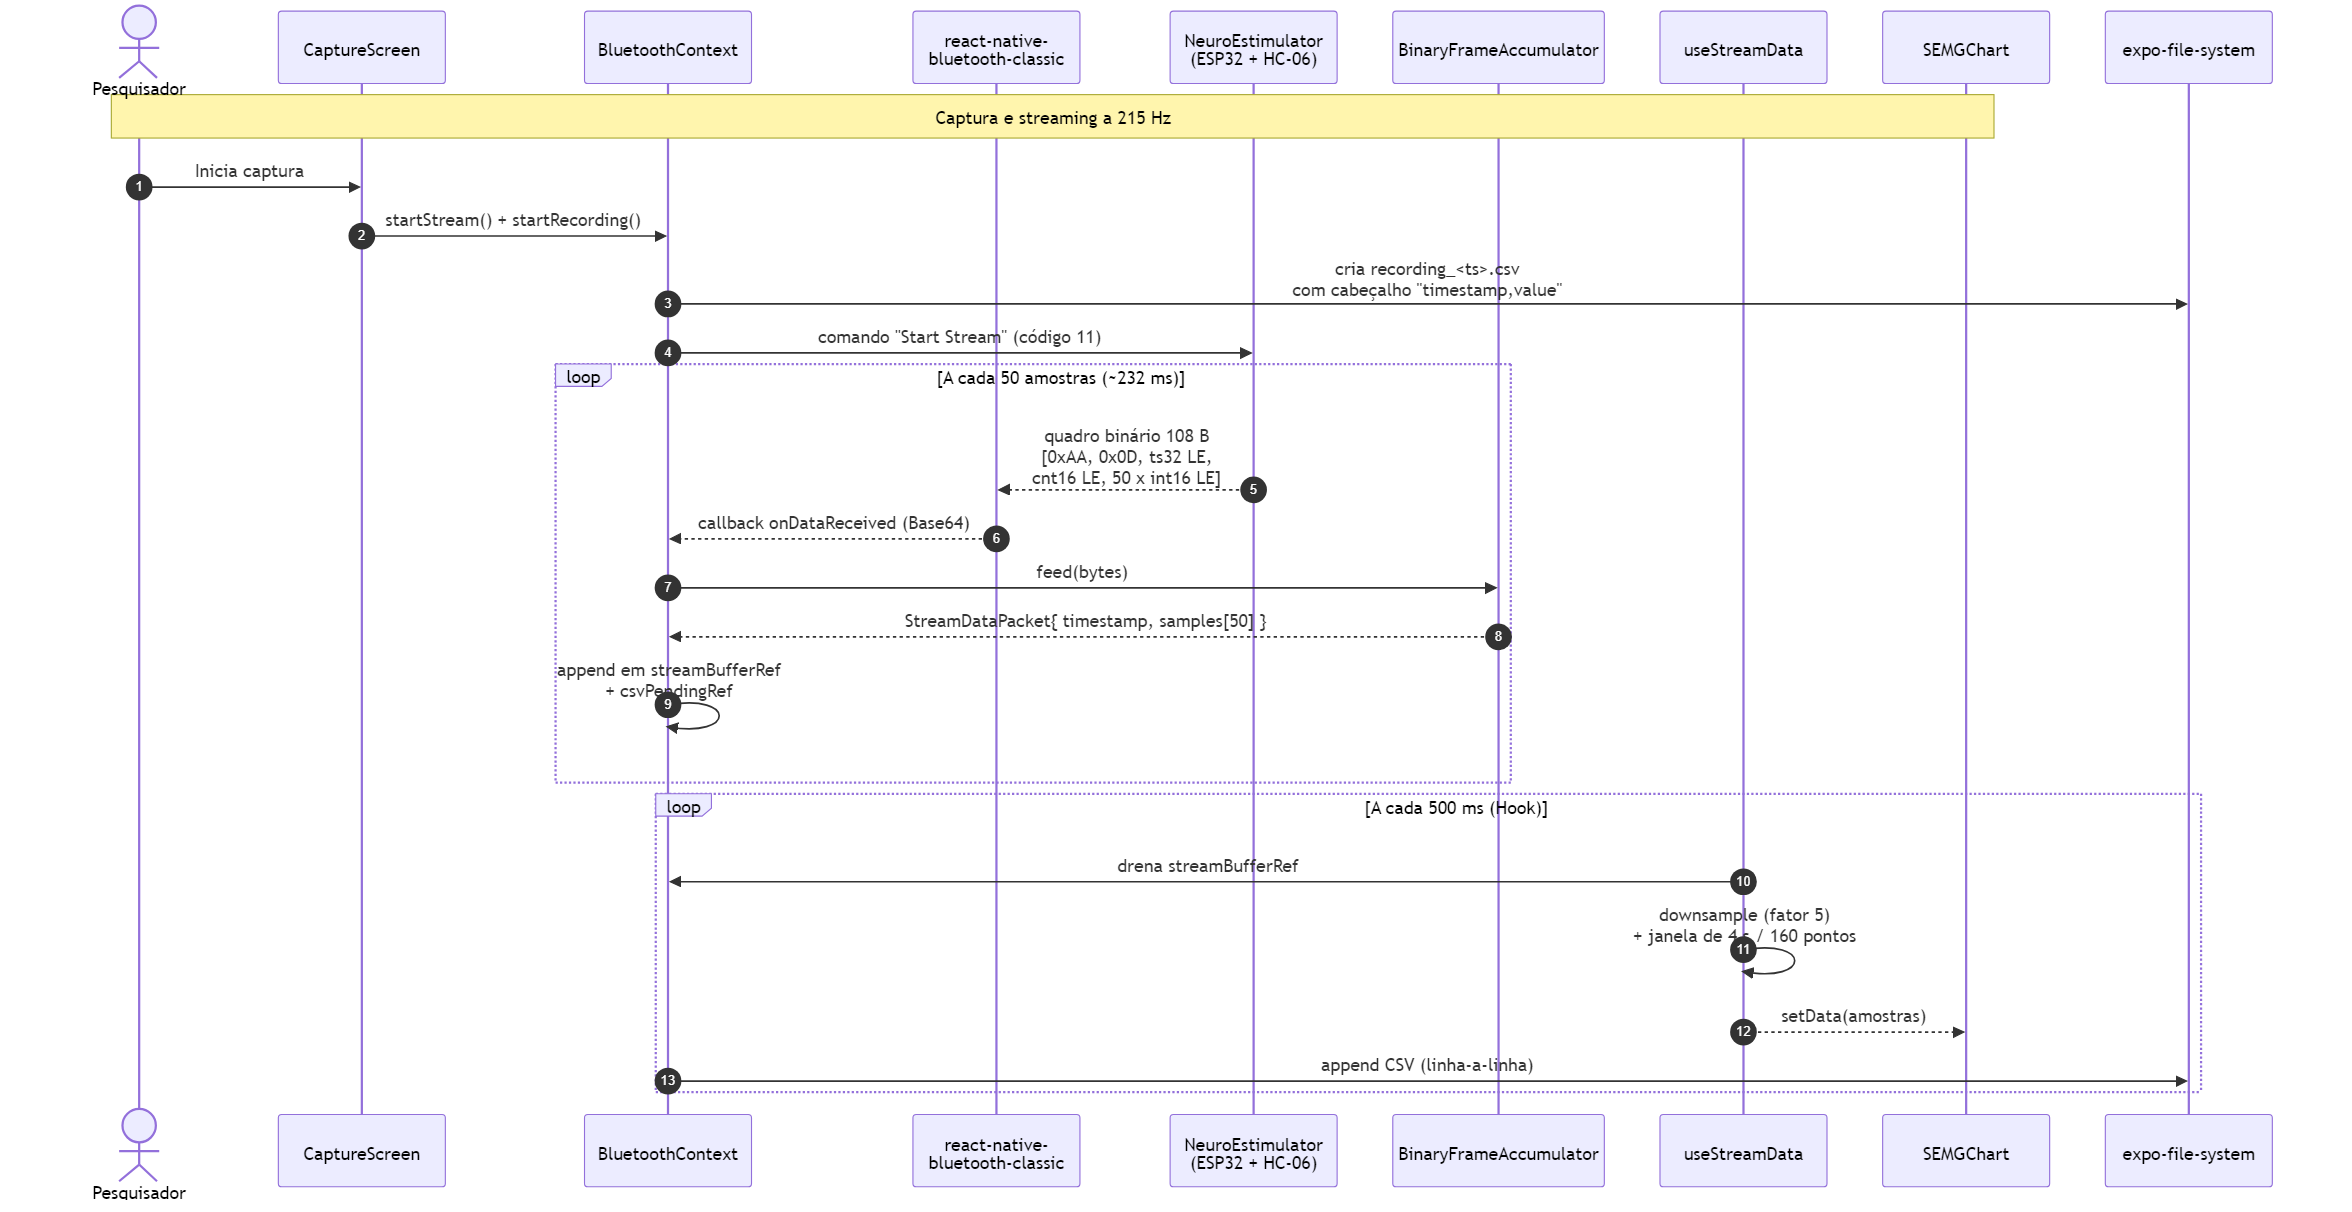
\includegraphics[scale=0.5]{figuras/Desenvolvimento/IRISMobile/fluxo-bt-streaming-2-captura.png}
\fonte{}
\end{figure}

\begin{figure}[htpb]
\caption{IRIS \textit{Mobile} --- encerramento da captura e recuperação de desconexão Bluetooth.}
\label{fig:IRISMobileFluxoCapturaEncerramento}
\centering
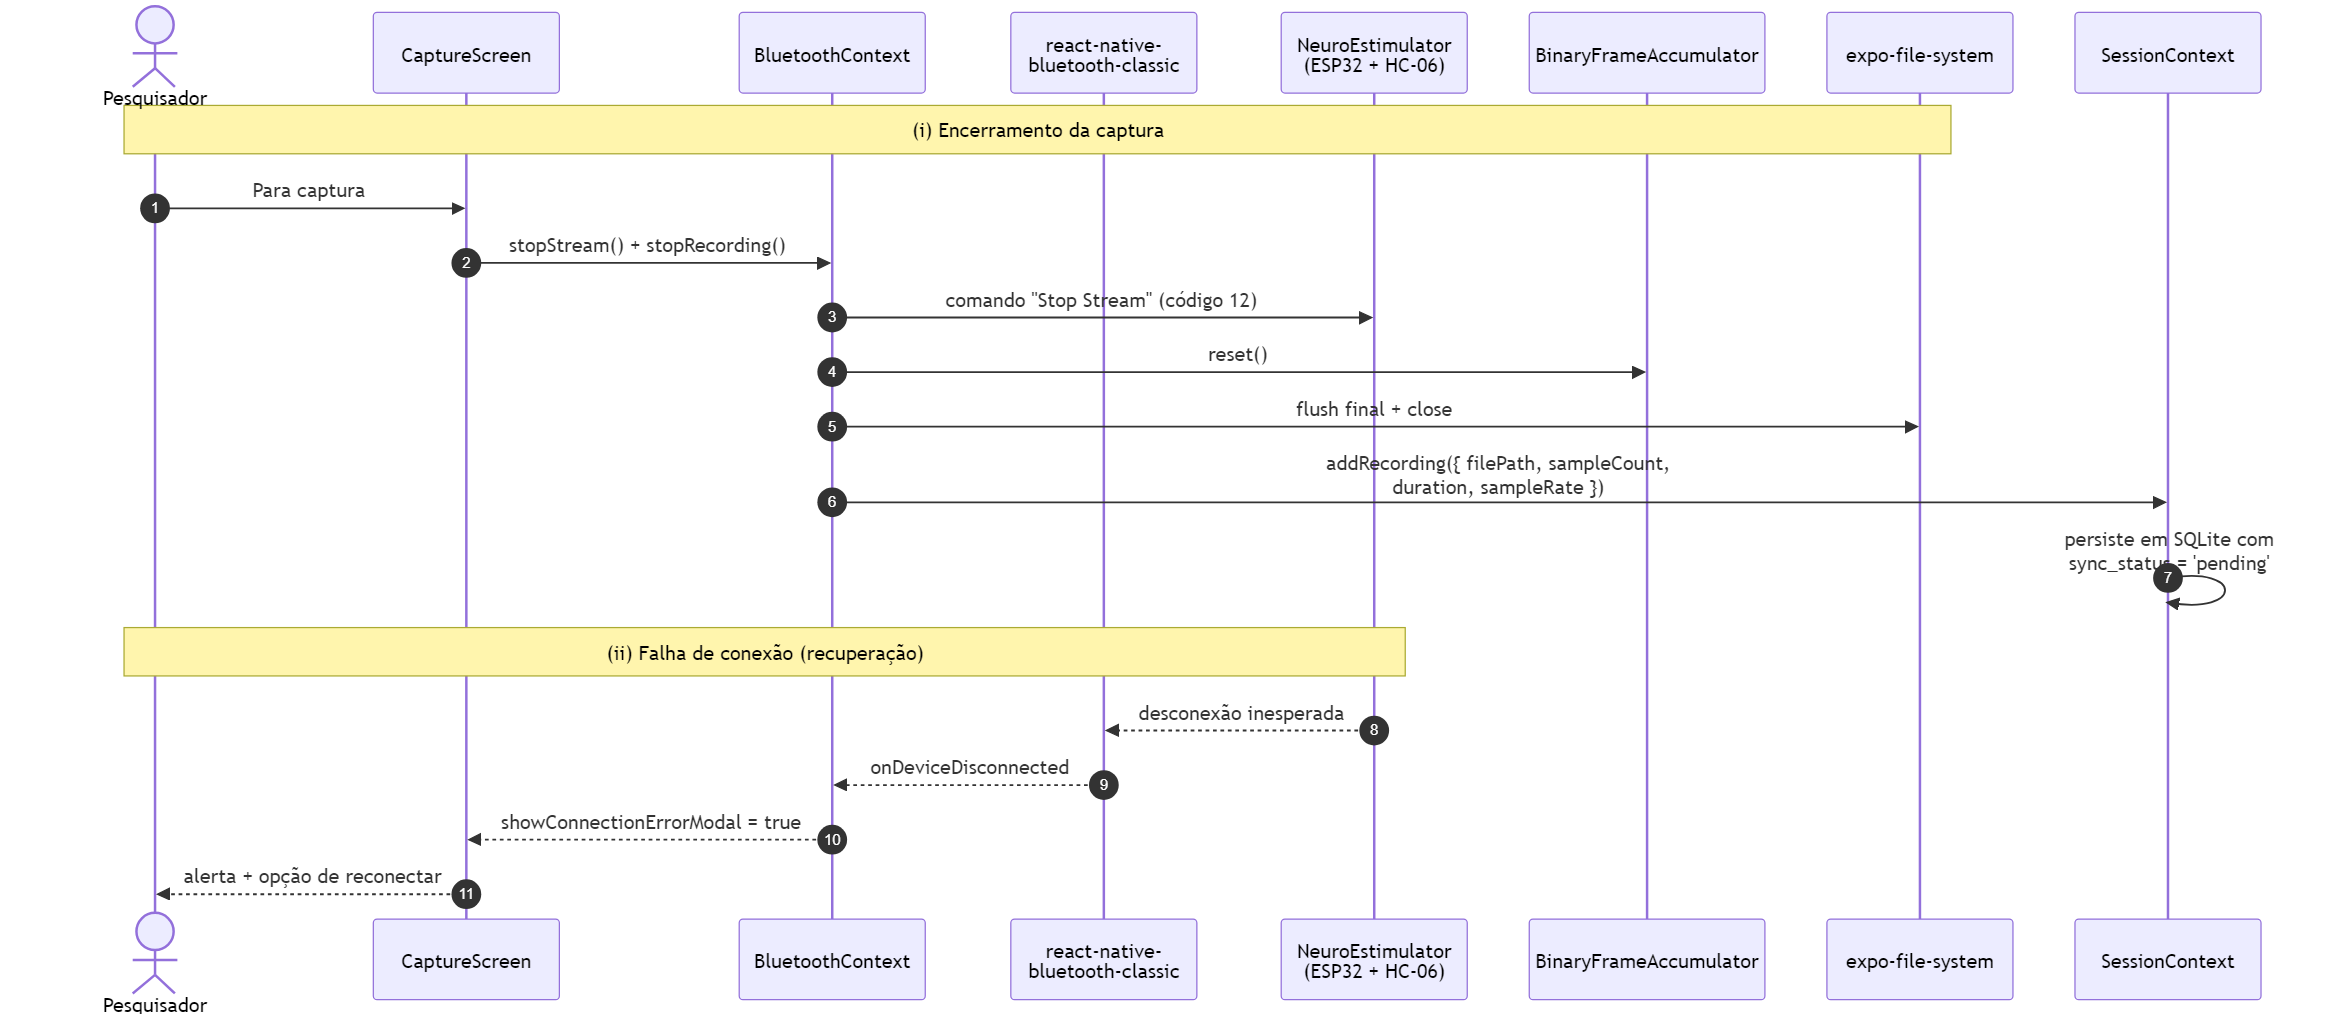
\includegraphics[scale=0.5]{figuras/Desenvolvimento/IRISMobile/fluxo-bt-streaming-3-encerramento.png}
\fonte{}
\end{figure}

\begin{figure}[htpb]
\caption{IRIS \textit{Mobile} --- geração local de sessão, gravação e anotações em modo \textit{offline-first}.}
\label{fig:IRISMobileFluxoSync}
\label{fig:IRISMobileFluxoSyncGeracao}
\centering
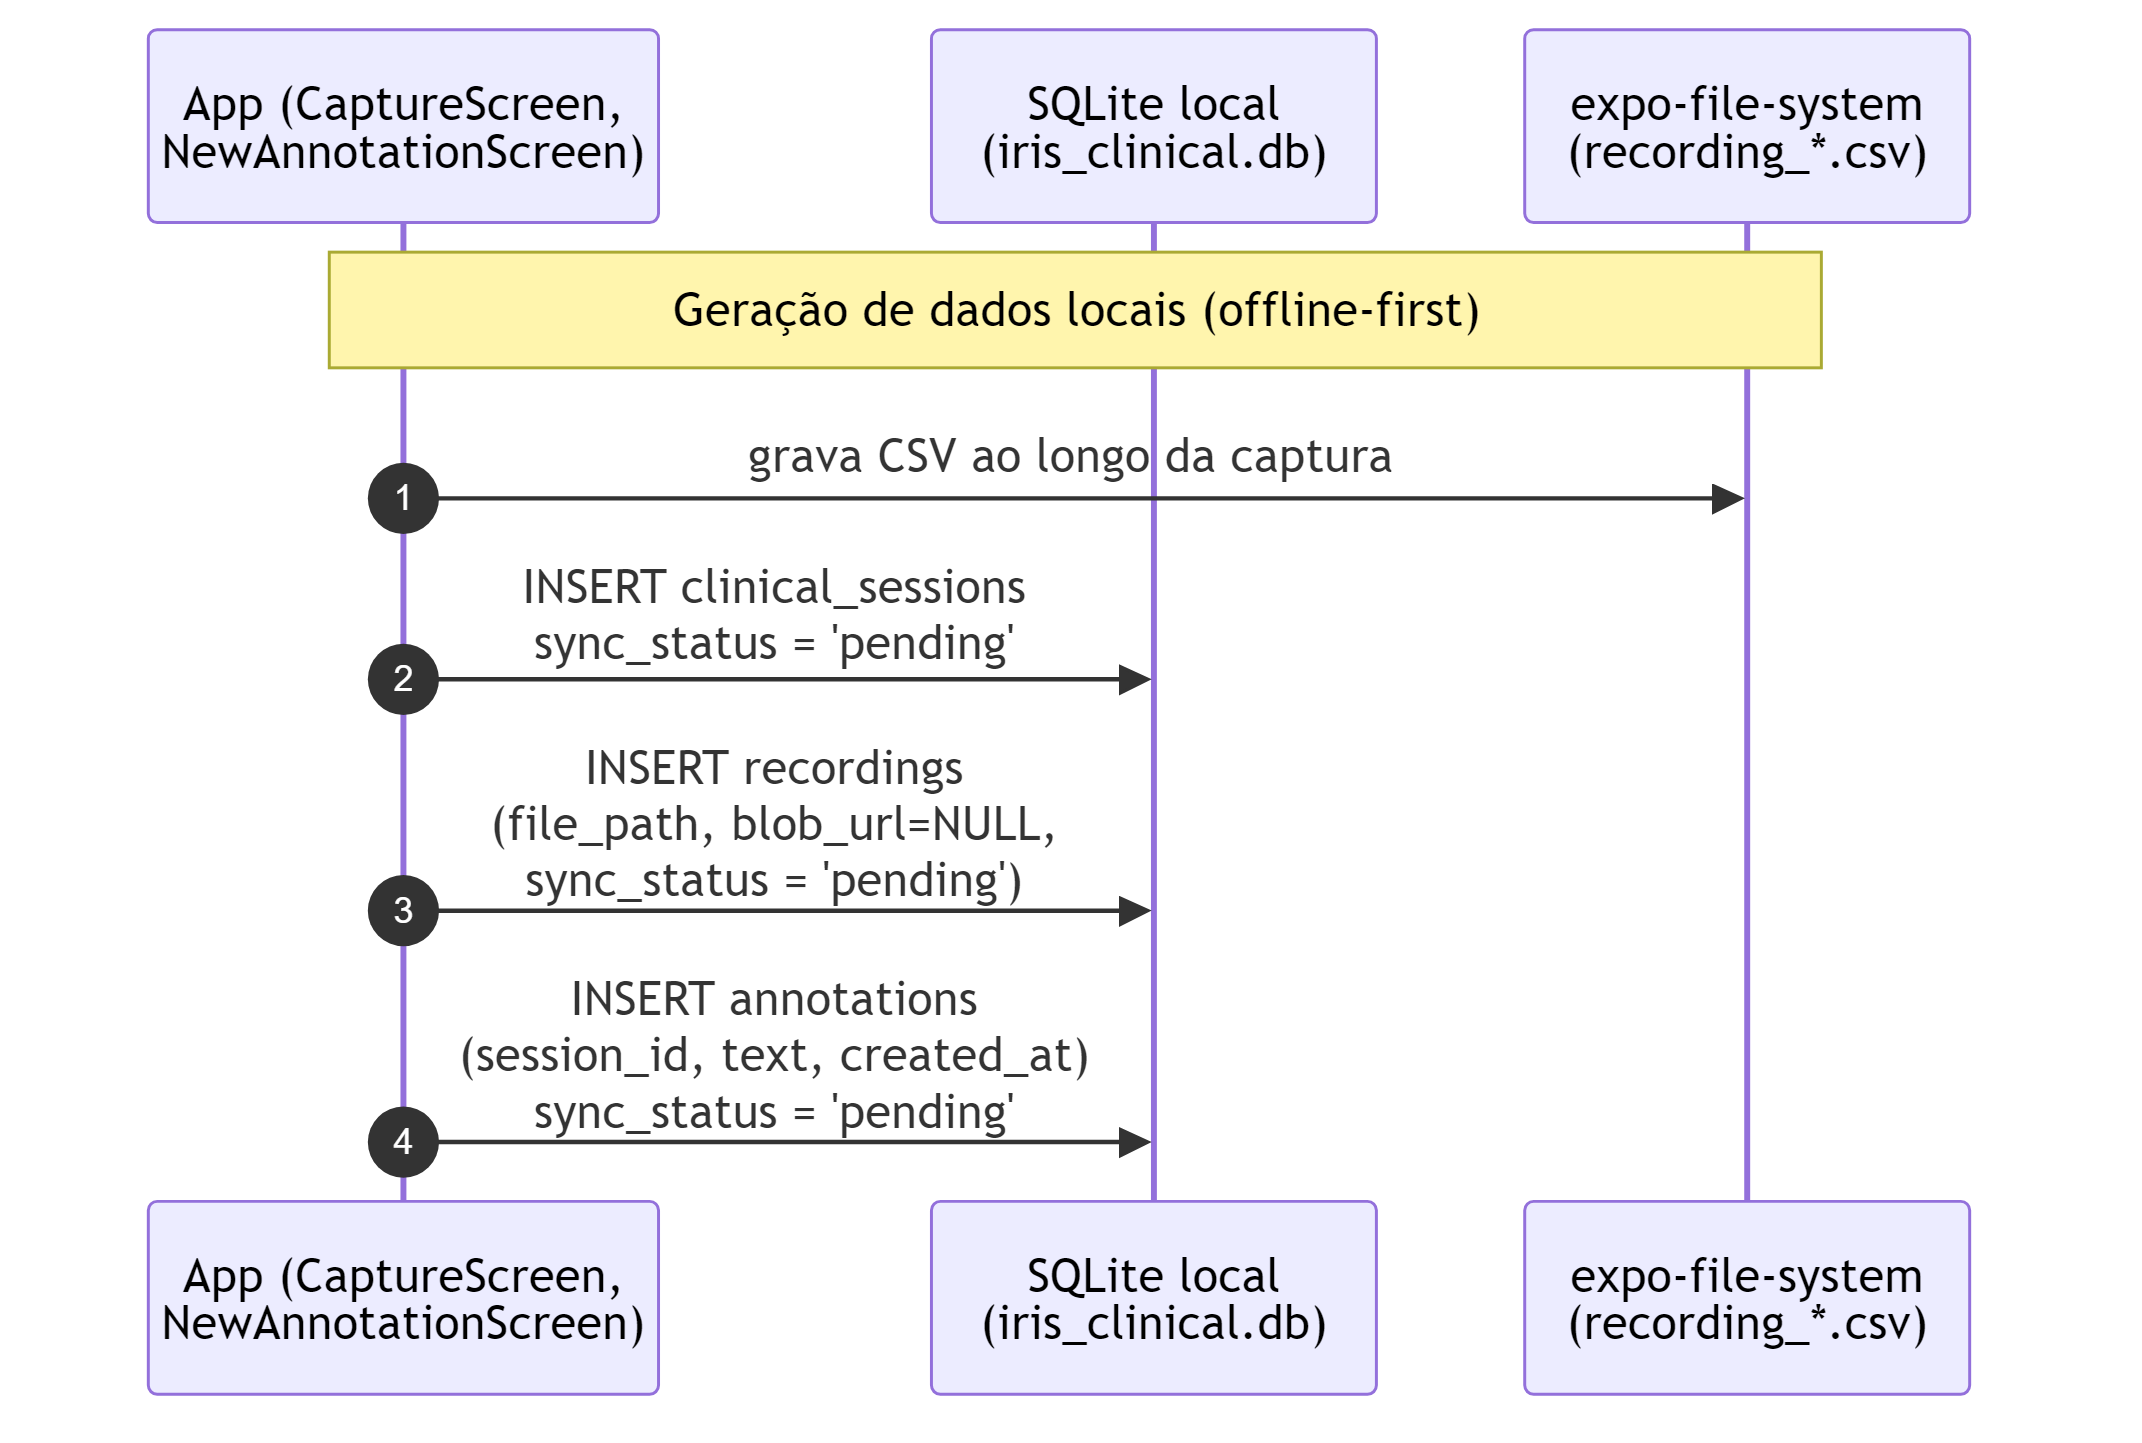
\includegraphics[scale=0.5]{figuras/Desenvolvimento/IRISMobile/fluxo-sync-mobile-1-geracao.png}
\fonte{}
\end{figure}

\begin{figure}[htpb]
\captionsetup{width=0.95\textwidth}
\caption{IRIS \textit{Mobile} --- ciclo periódico de \textit{upload} respeitando a ordem de dependências (sessão, gravação, anotação).}
\label{fig:IRISMobileFluxoSyncUpload}
\centering
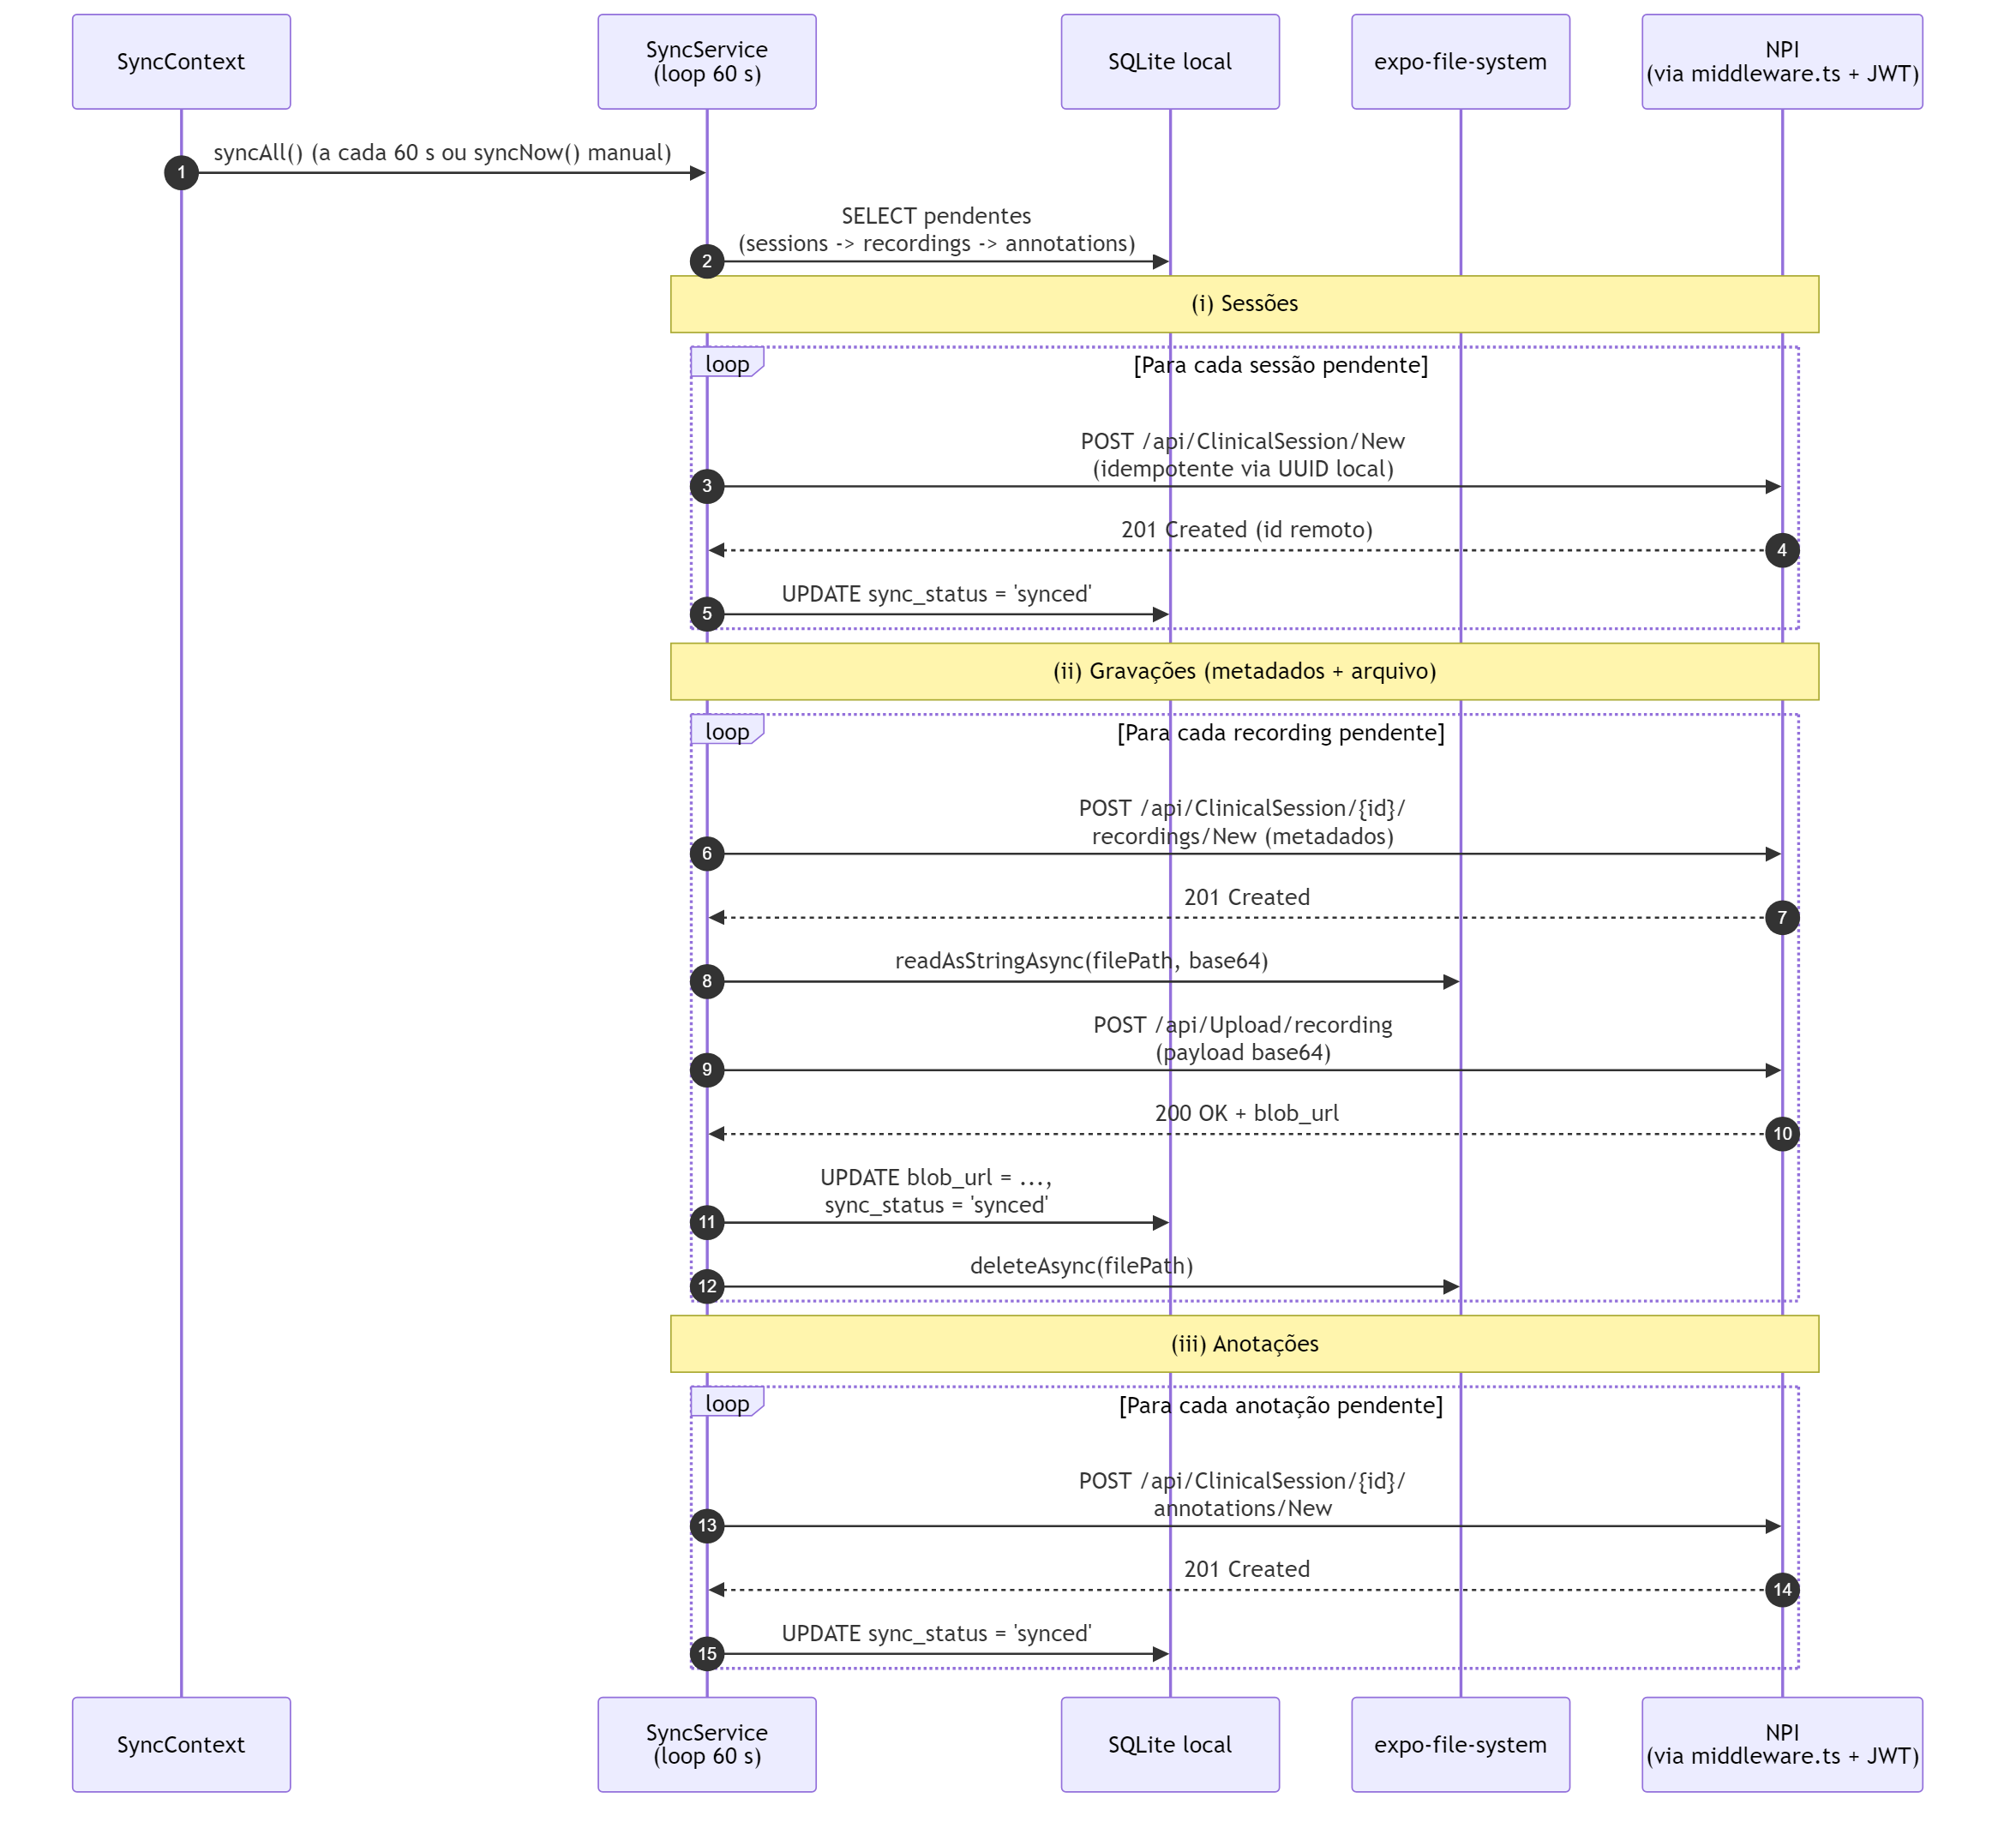
\includegraphics[scale=0.5]{figuras/Desenvolvimento/IRISMobile/fluxo-sync-mobile-2-upload.png}
\fonte{}
\end{figure}

\begin{figure}[htpb]
\caption{IRIS \textit{Mobile} --- tratamento do resultado da sincronização e atualização do \textit{badge} na \texttt{HistoryScreen}.}
\label{fig:IRISMobileFluxoSyncResultado}
\centering
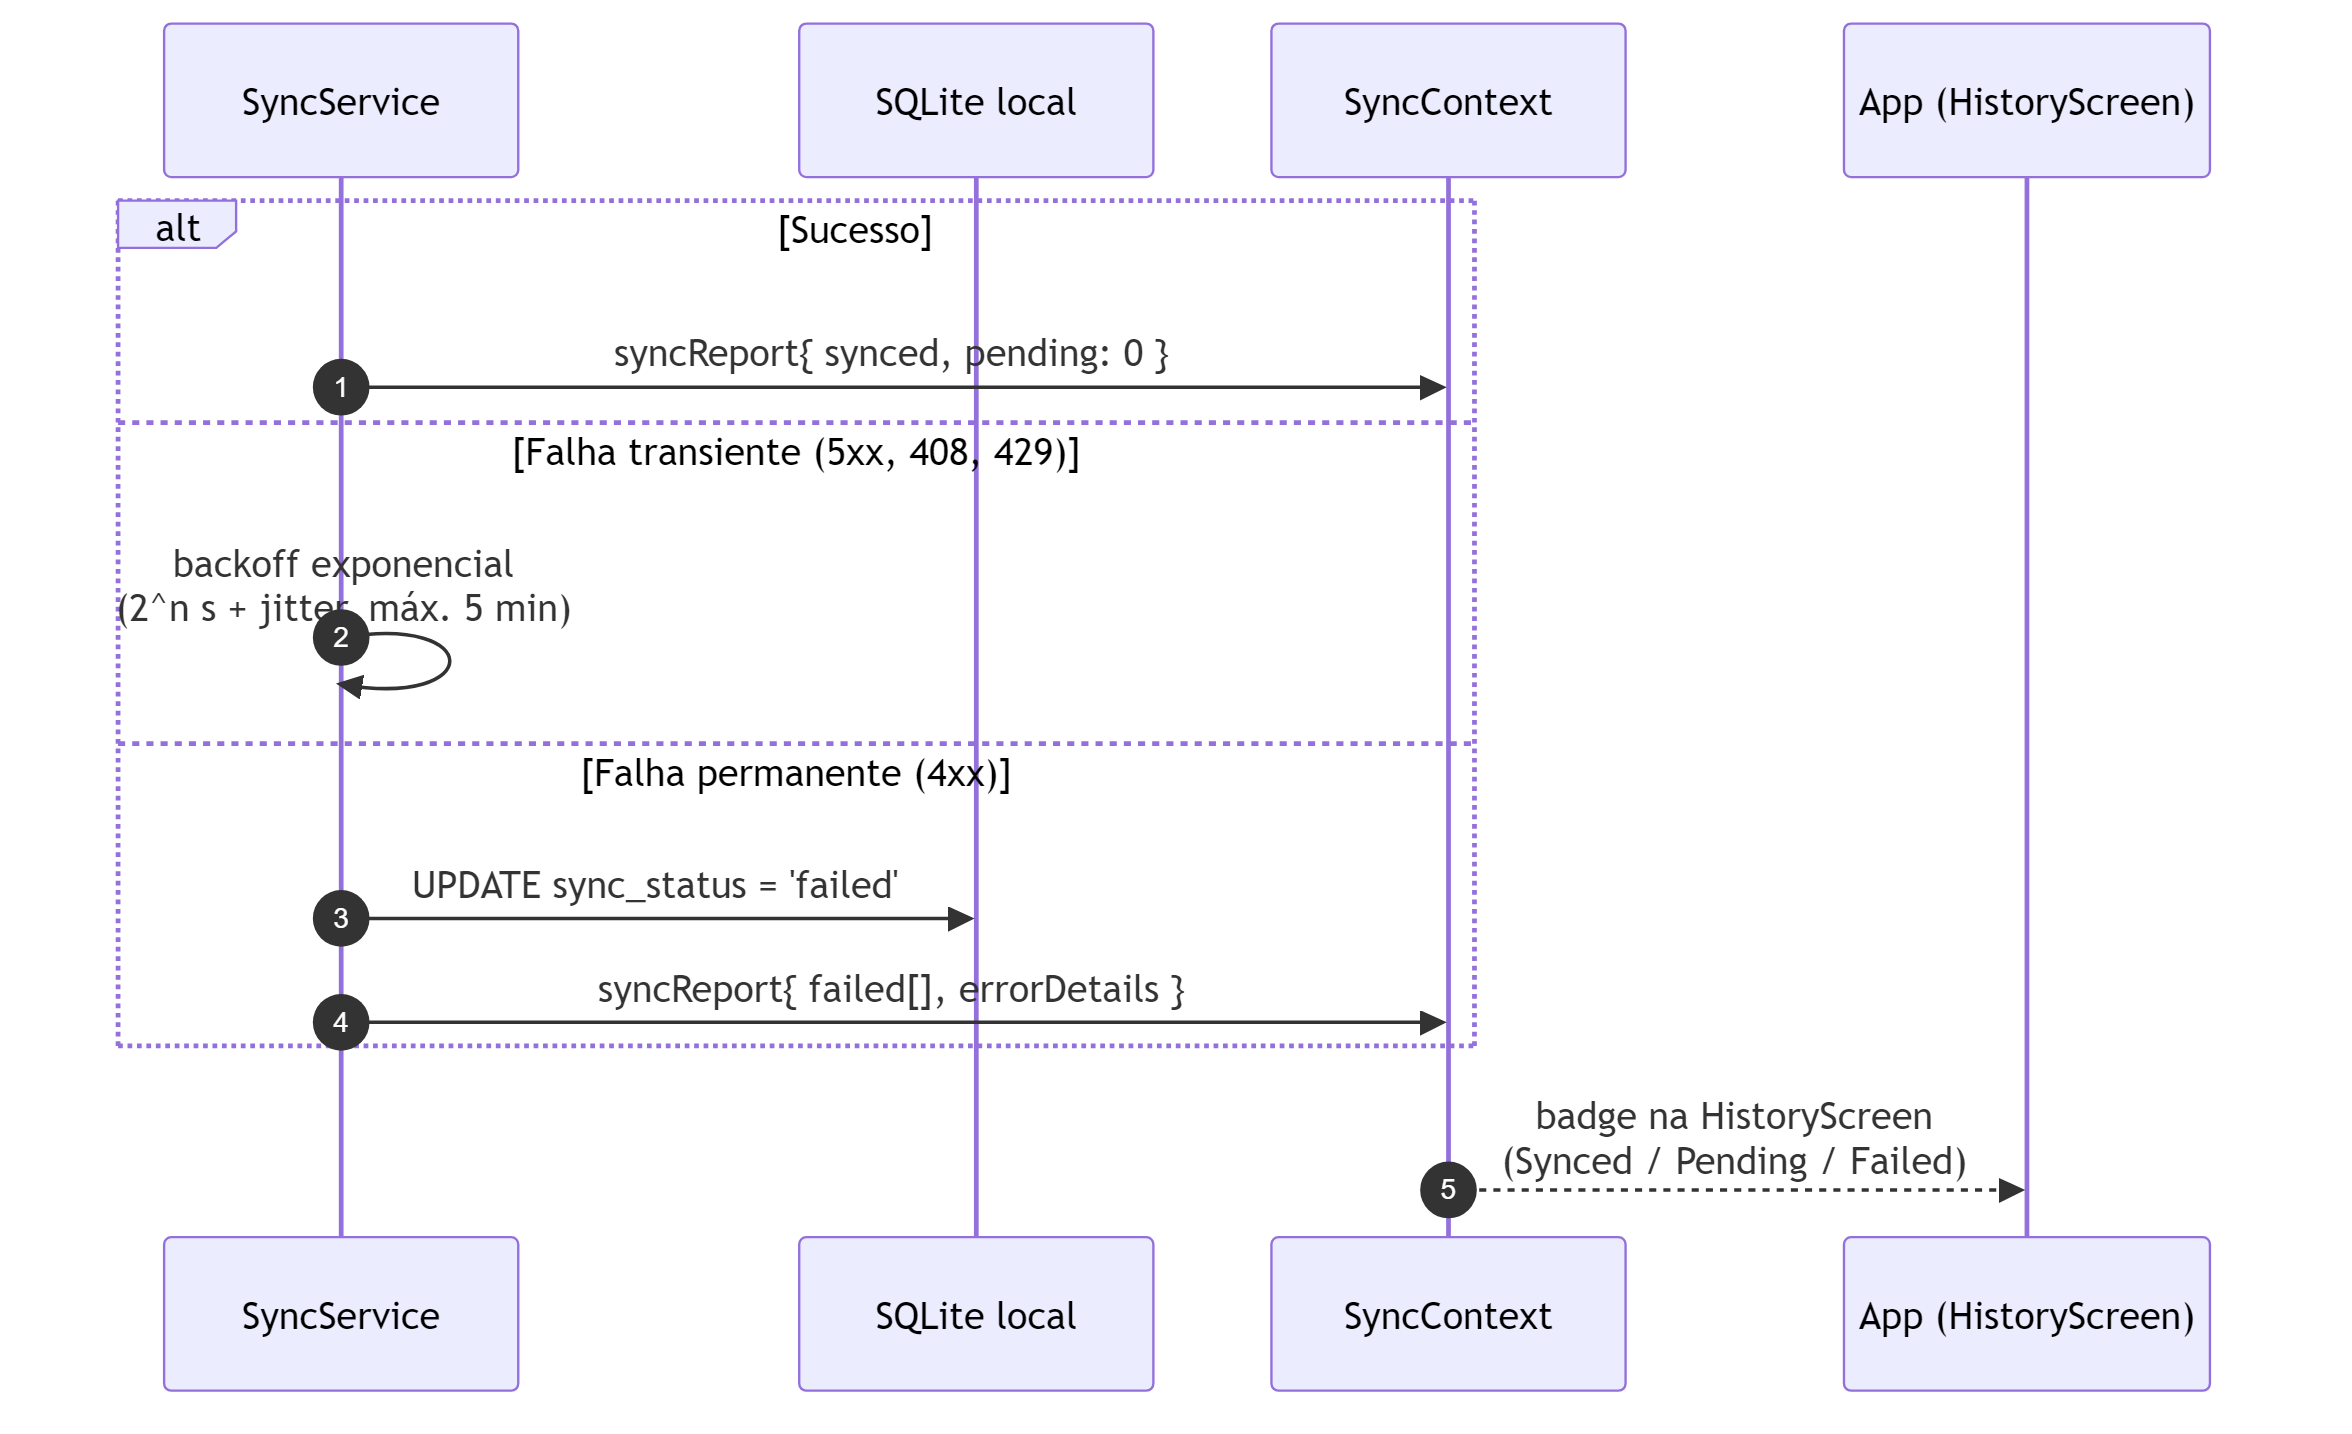
\includegraphics[scale=0.5]{figuras/Desenvolvimento/IRISMobile/fluxo-sync-mobile-3-resultado.png}
\fonte{}
\end{figure}

\begin{figure}[htpb]
\caption{IRIS \textit{Mobile} --- criação local da anotação clínica e persistência em SQLite.}
\label{fig:IRISMobileFluxoRotulagem}
\label{fig:IRISMobileFluxoRotulagemCriacao}
\centering
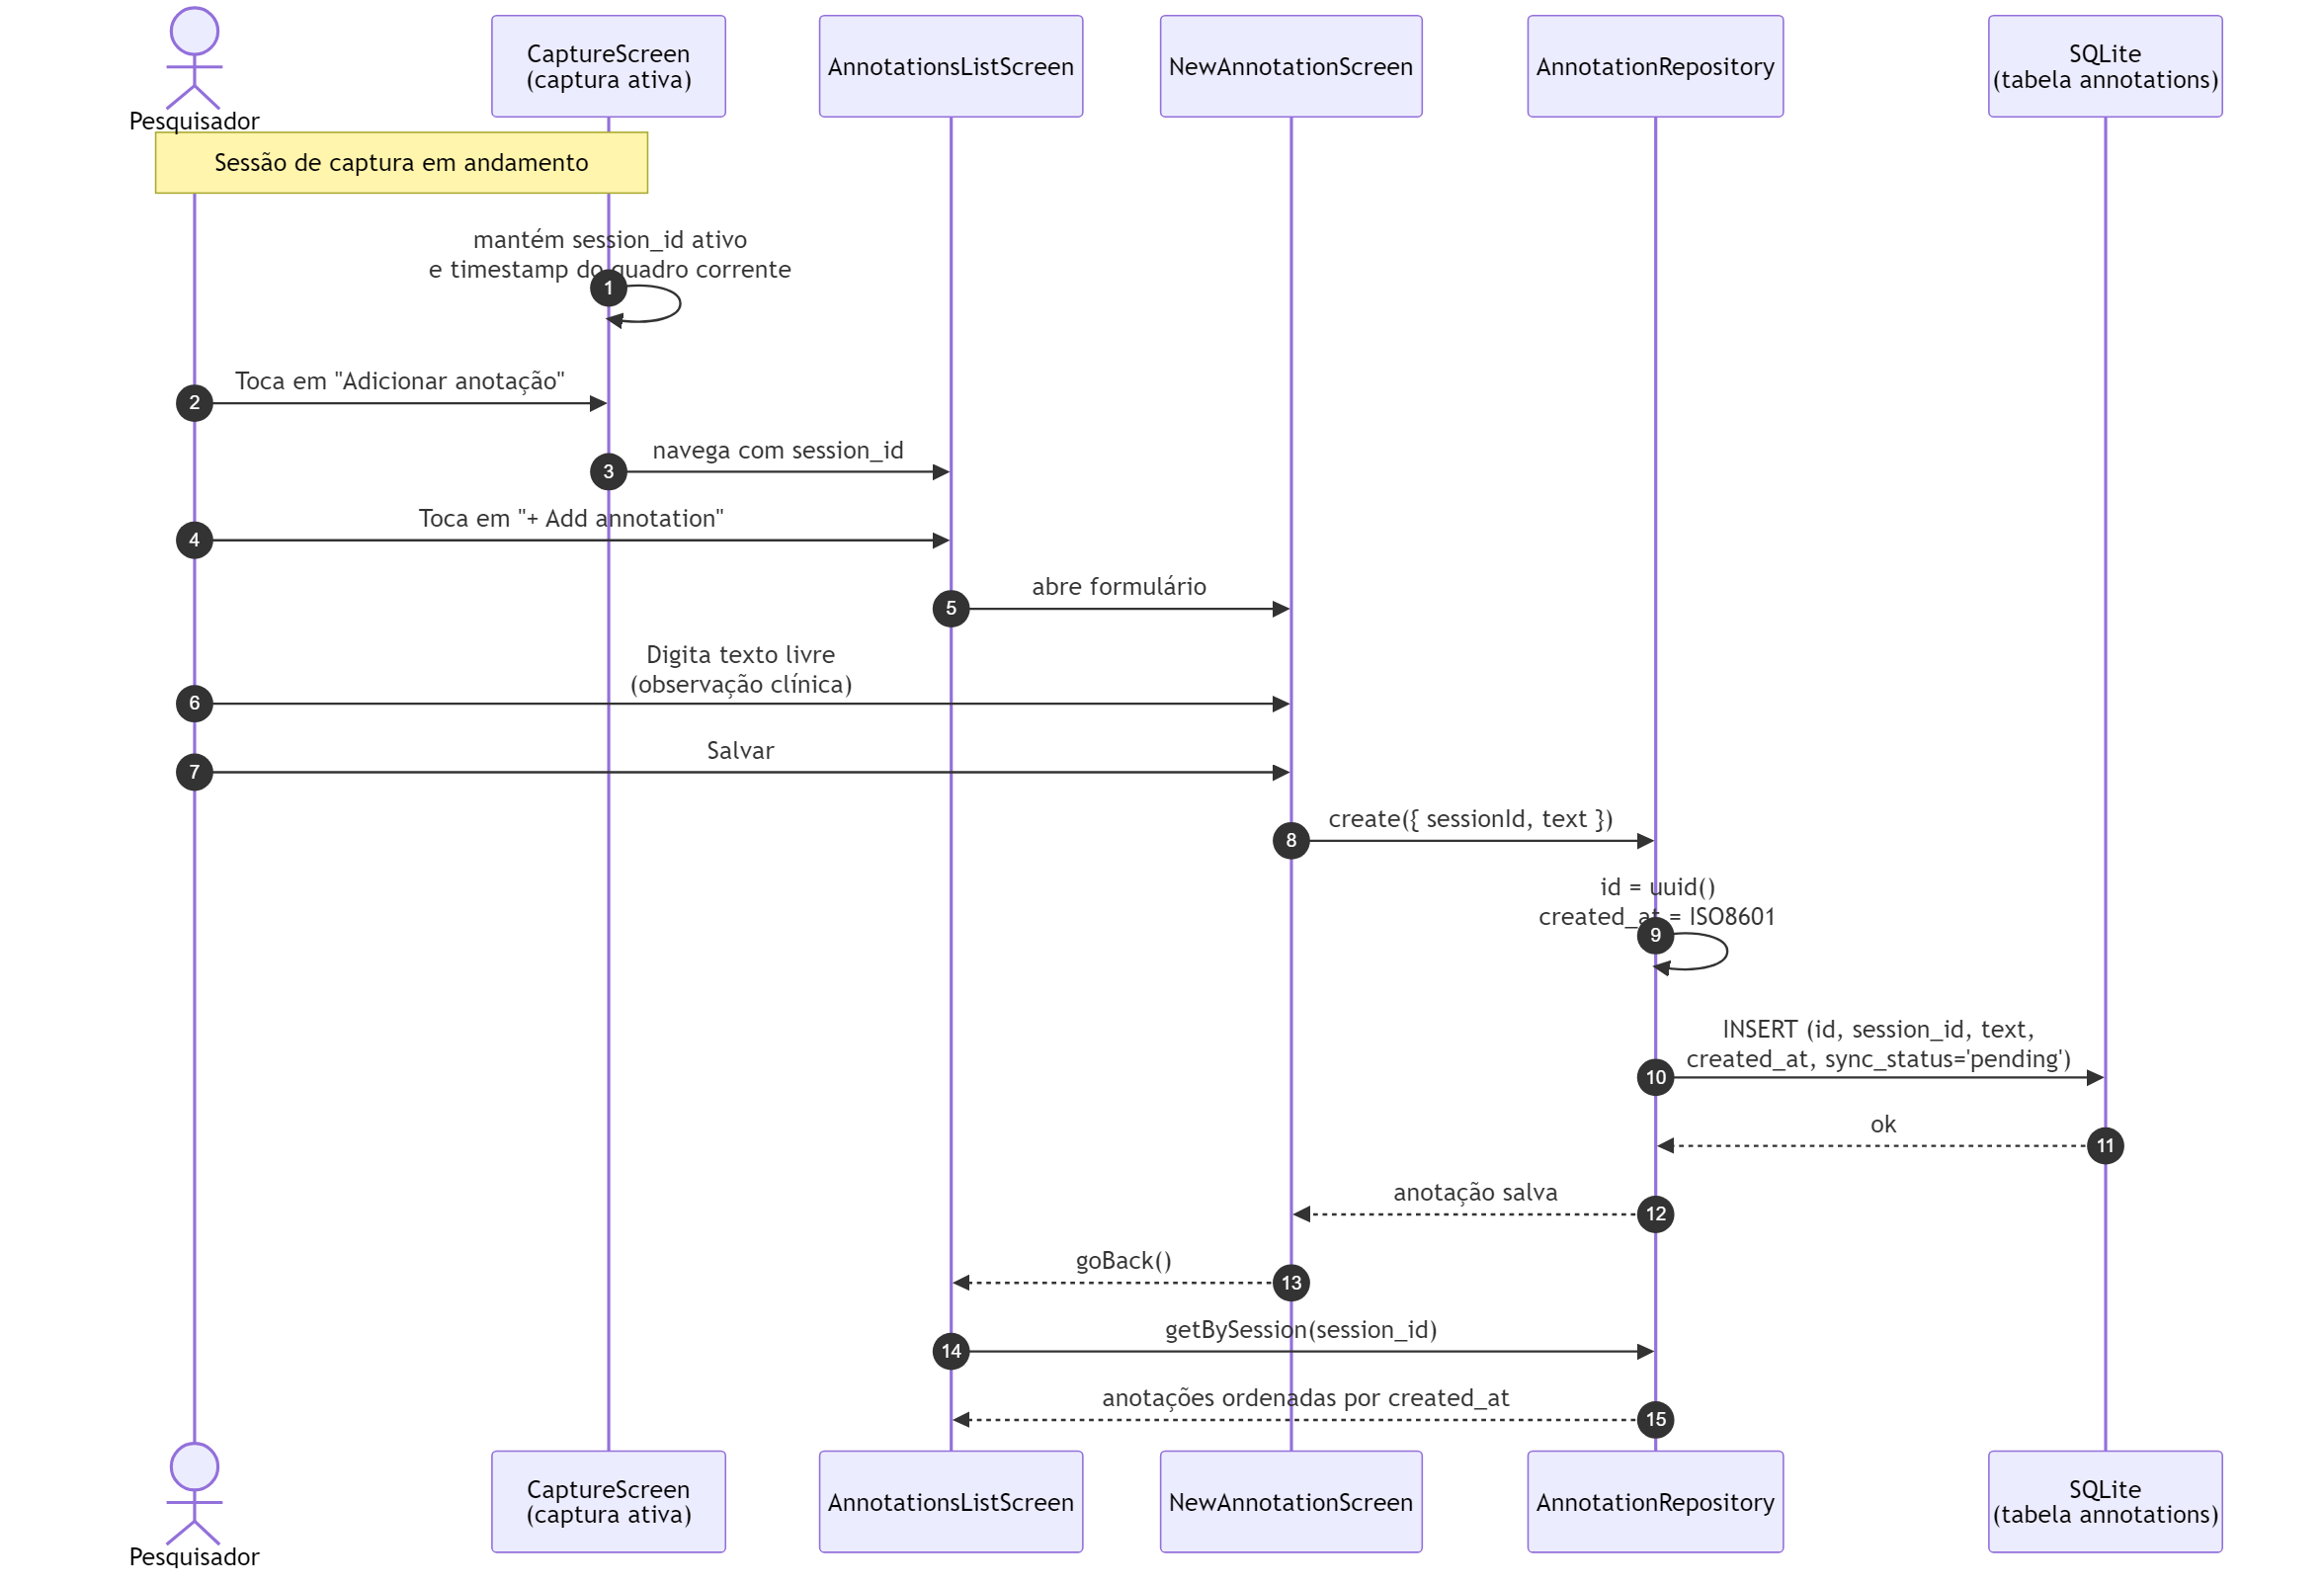
\includegraphics[scale=0.5]{figuras/Desenvolvimento/IRISMobile/fluxo-rotulagem-1-criacao.png}
\fonte{}
\end{figure}

\begin{figure}[htpb]
\caption{IRIS \textit{Mobile} --- envio assíncrono das anotações ao NPI pelo \texttt{SyncService}.}
\label{fig:IRISMobileFluxoRotulagemEnvio}
\centering
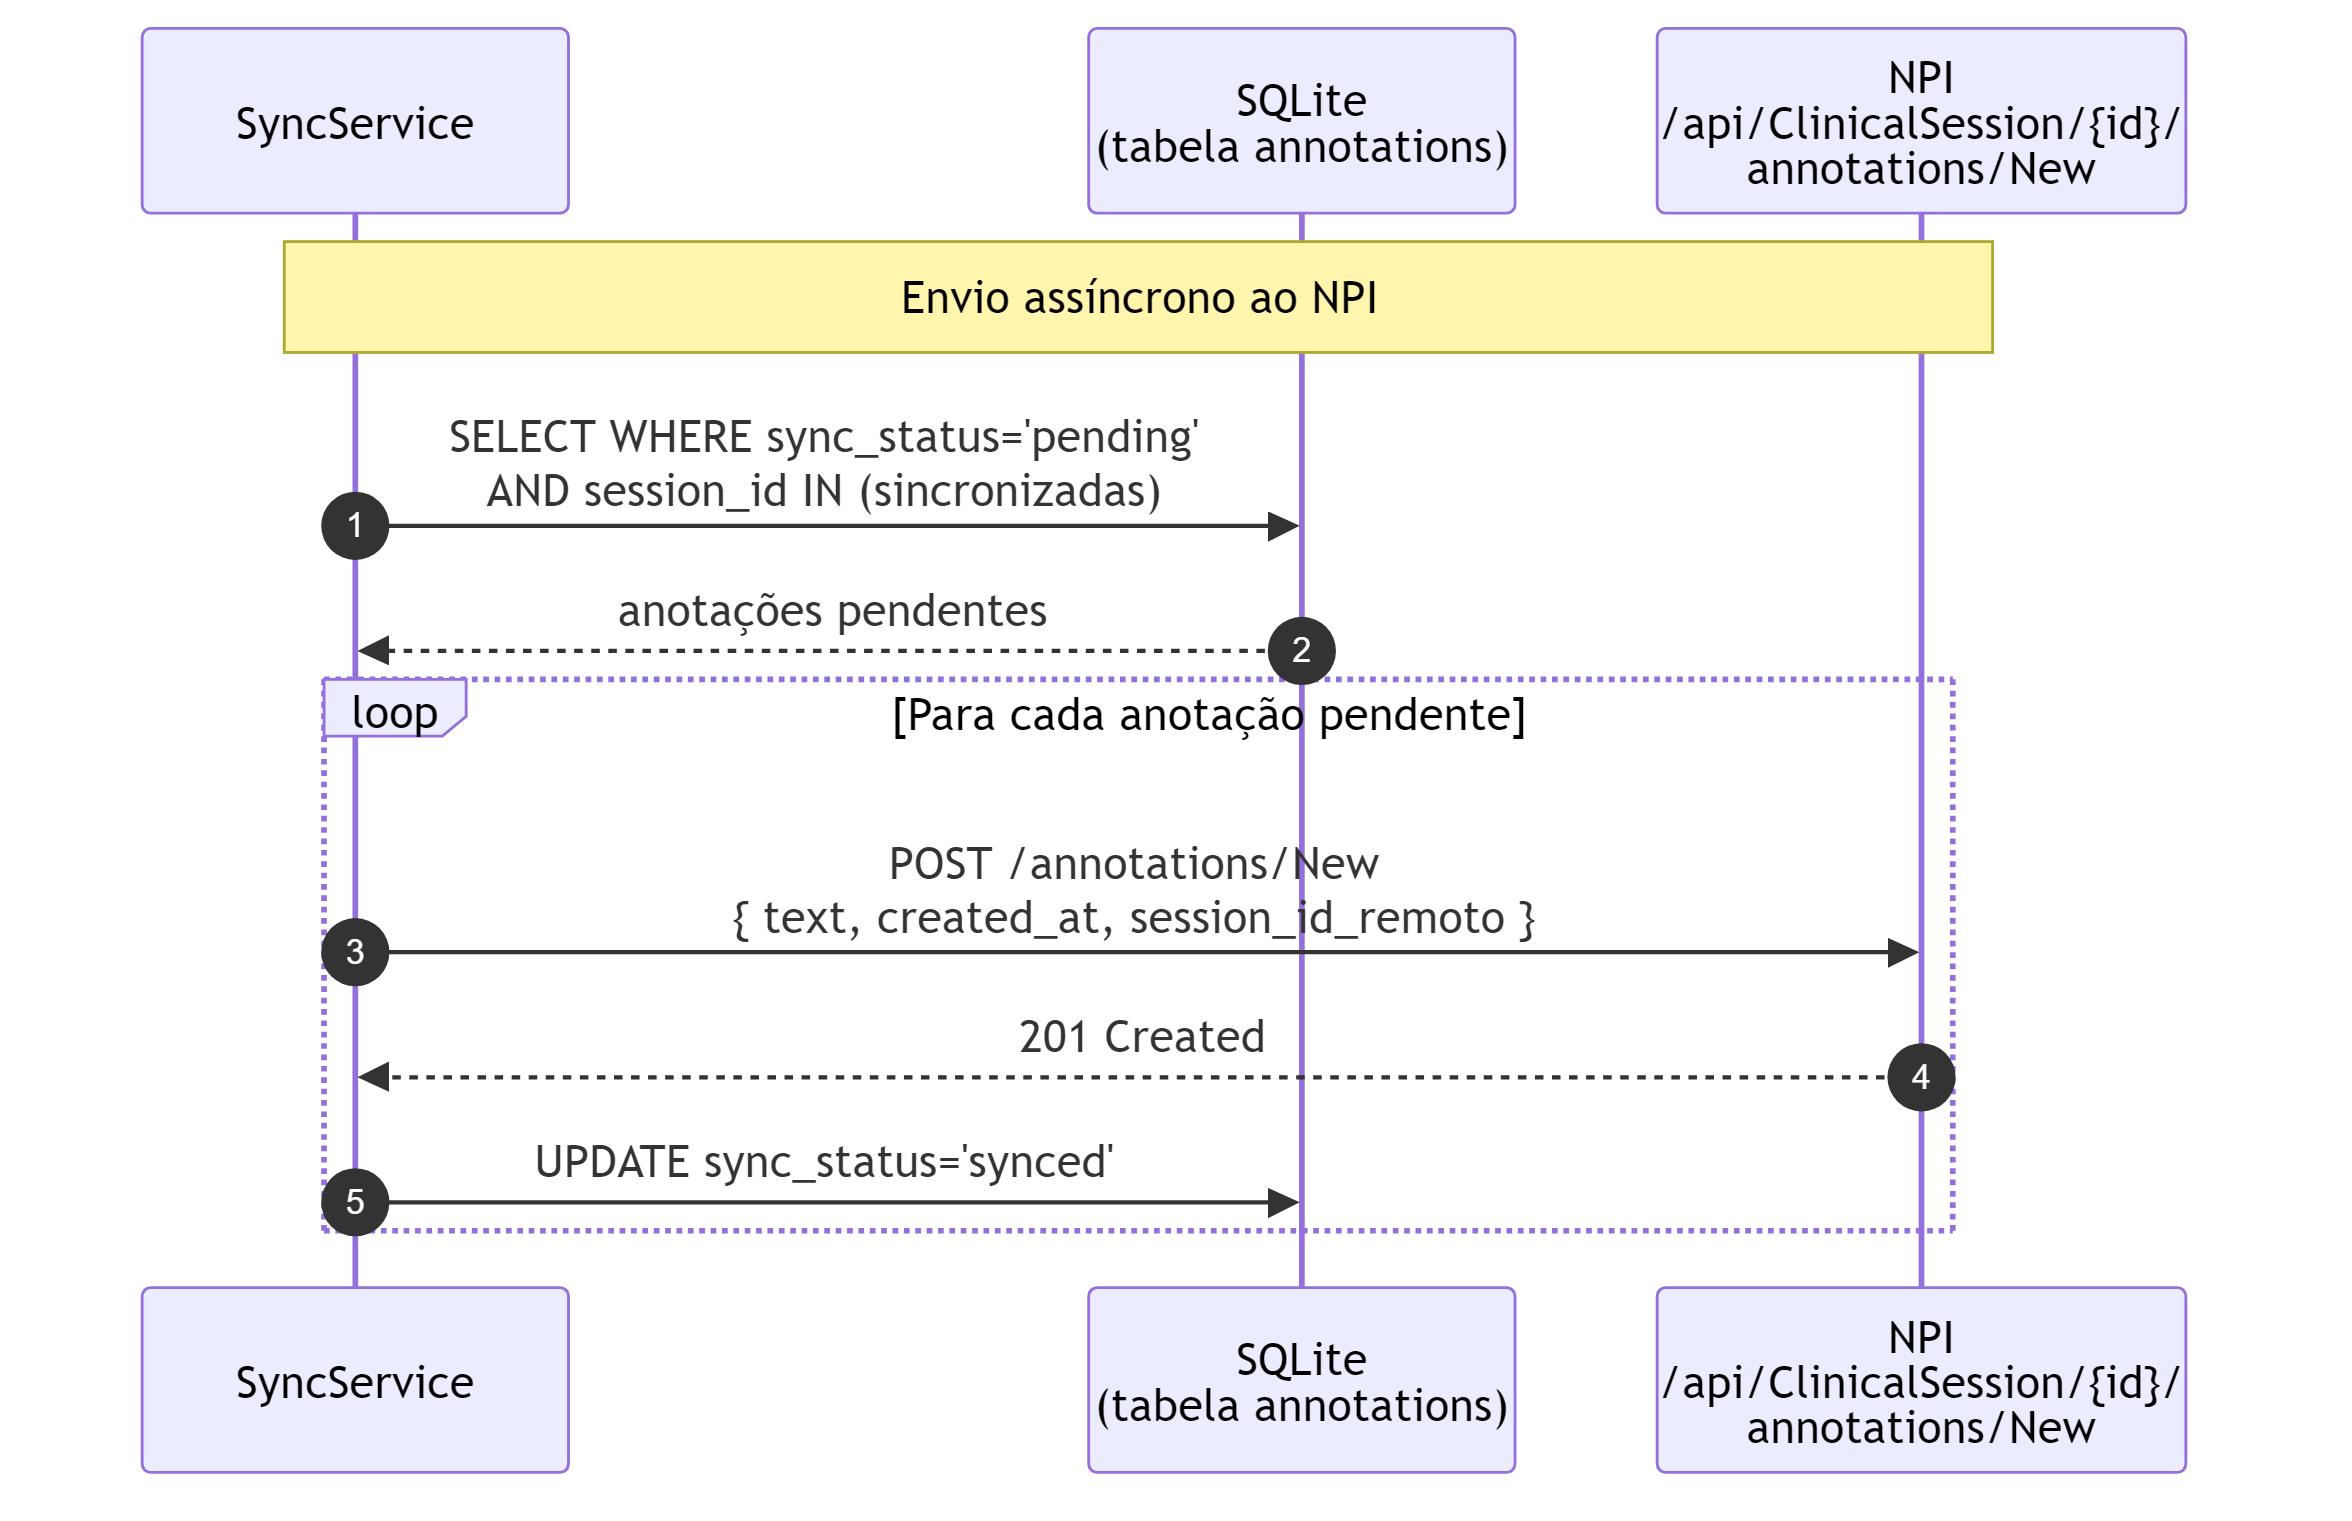
\includegraphics[scale=0.5]{figuras/Desenvolvimento/IRISMobile/fluxo-rotulagem-2-envio.png}
\fonte{}
\end{figure}

% ----------------------------------------------------------------------
\section{Streaming Bluetooth do NeuroEstimulator}\label{sec:apendiceSeqStreaming}
% ----------------------------------------------------------------------

A Figura~\ref{fig:protocoloStreaming} resume o diálogo completo entre o IRIS \textit{Mobile}, o tratador de mensagens, as tarefas internas do \textit{firmware} e o canal Bluetooth durante uma sessão de aquisição, em complemento à discussão da Subseção~\ref{subsubsec:NEProtocolo}. O diagrama evidencia a coexistência entre o protocolo de comandos em JSON --- empregado para abertura e encerramento do \textit{streaming} --- e o fluxo binário compacto de pacotes de 108~\textit{bytes} emitidos autonomamente pelo \textit{firmware} a cada cinquenta amostras coletadas, padrão que substituiu o modelo legado de comando-resposta para o canal de dados.

\begin{figure}[htpb]
\caption{Diagrama de sequência do \textit{streaming} de sEMG entre o IRIS \textit{Mobile} e o \textit{firmware} adaptado.}
\label{fig:protocoloStreaming}
\centering
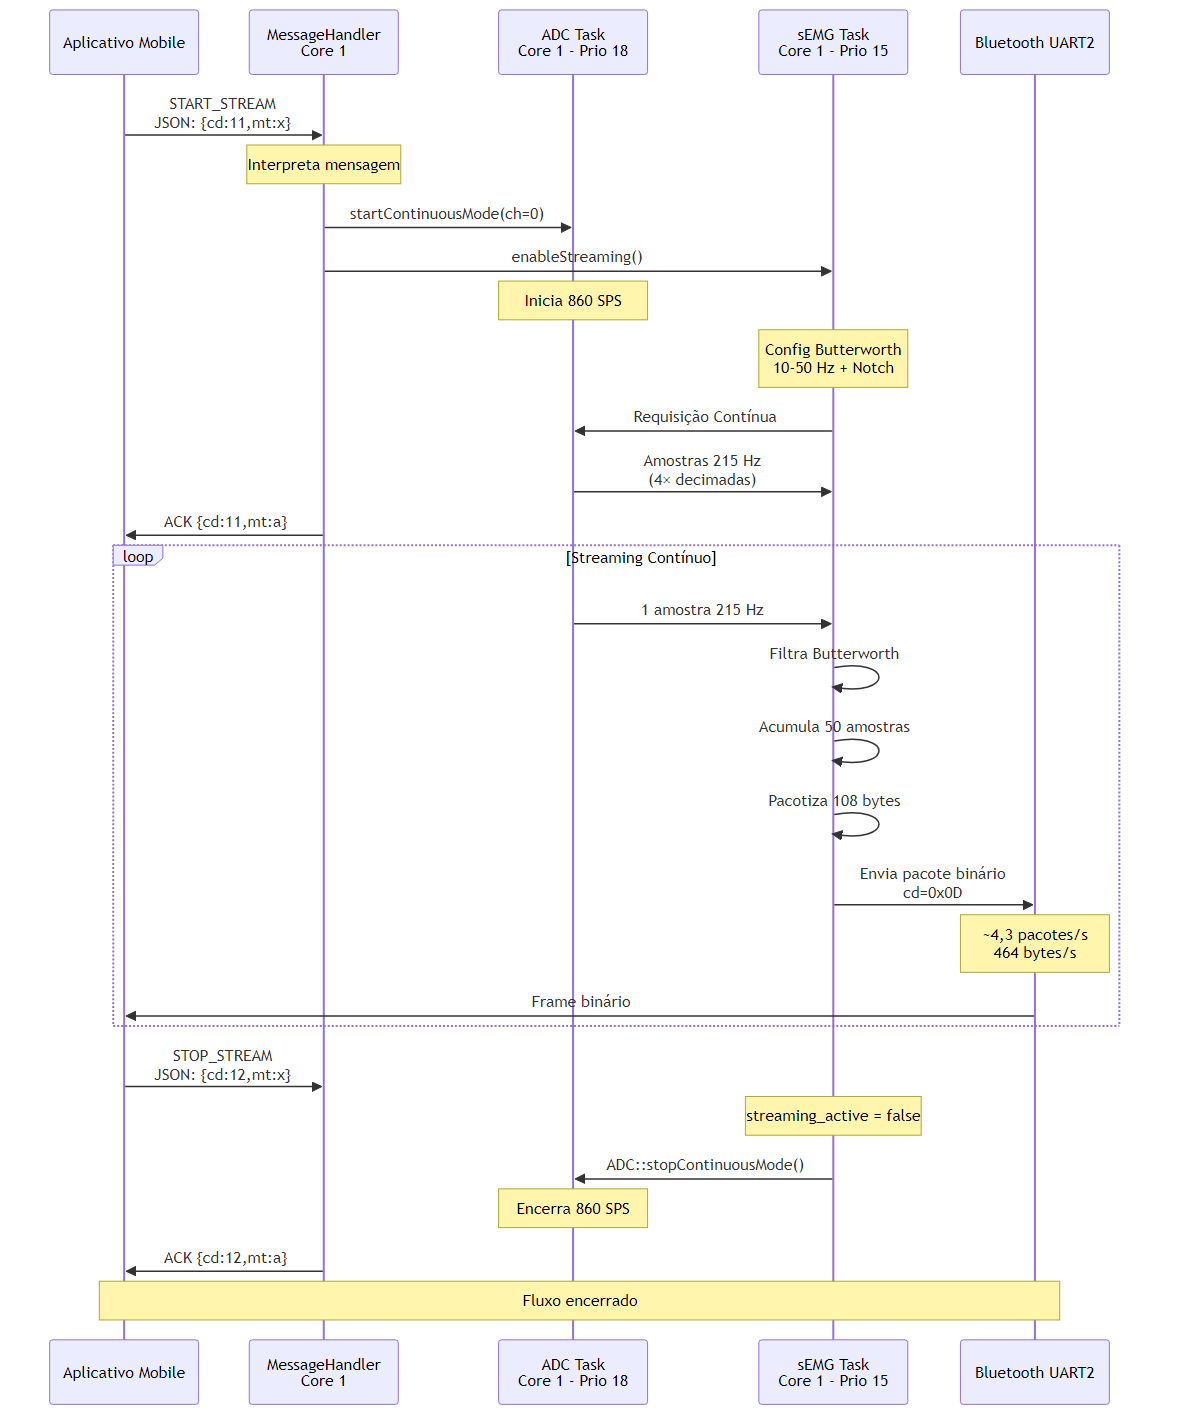
\includegraphics[width=\textwidth]{figuras/Desenvolvimento/NeuroEstimulator/protocolo-streaming.png}
\fonte{}
\end{figure}
